\documentclass[aspectratio=169]{beamer}
\usepackage{color,amsmath}
\usepackage{subfigure}
\usepackage{booktabs}
\usepackage{framed}
\usepackage{comment}
\usepackage{url}

\usepackage{hyperref}
\hypersetup{
    colorlinks=true,
    linkcolor=blue,
    filecolor=magenta,      
    urlcolor=cyan,
}

%%%%%%%%%%%%%%%%%%%%%%%%%%
\title[]{\textcolor{gray}{[Survey research in the digital age], [Probability and non-probability sampling], [Computer-administered interviews],} [Combining surveys and big data]\textcolor{gray}{, [Additions and extensions]}}
\author[]{Matthew J. Salganik\\Department of Sociology\\Princeton University}
\date[]{%Summer Institutes in Computational Social Science\\2020
%\vfill
%\begin{flushleft}
%{\scriptsize
%The Summer Institutes in Computational Social Science is supported by grants from the Russell Sage Foundation and the Alfred P. Sloan Foundation.}
%\end{flushleft}
\begin{flushright}

\includegraphics[width=0.1\textwidth]{figures/cc-by.png}
\end{flushright}
}
\begin{document}
%%%%%%%%%%%%%%%%%%%%%%%%%%
\frame{\titlepage}
%%%%%%%%%%%%%%%%%%%%%%%%%%
\begin{frame}

\begin{columns}
\begin{column}{.40\textwidth}
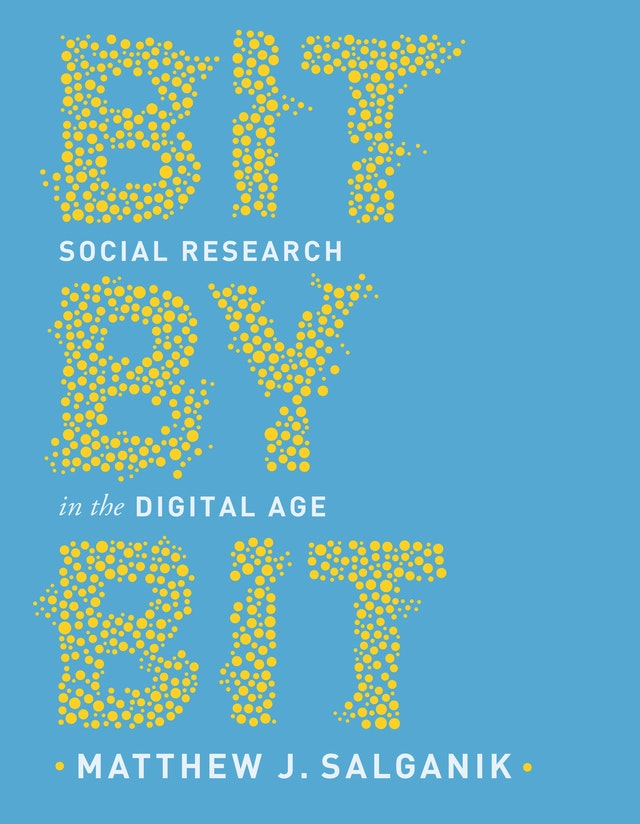
\includegraphics[width=\textwidth]{figures/salganik_bit_2018_cover}
\end{column}%

\hfill%

\begin{column}{.60\textwidth}
1) Introduction \\
2) Observing behavior \\
\textcolor{blue}{3) Asking questions} \\
4) Running experiments \\
5) Mass collaboration \\
6) Ethics \\
7) The future \\
\end{column}%
\end{columns}

\end{frame}
%%%%%%%%%%%%%%%%%%%%%%%%%%
\begin{frame}

\begin{center}
\small{
\begin{tabular}{ l c c c}
           & Sampling & Interviews & Data environment\\
\hline
1st era & Area probability & Face-to-face & Stand-alone \\
2nd era & \parbox[t]{3cm}{\centering Random digital dial\\probability} & Telephone & Stand-alone \\
3rd era & Non-probability & Computer-administered & \textcolor{blue}{Linked} \\
\end{tabular}
}
\end{center}

\end{frame}
%%%%%%%%%%%%%%%%%%%%%%%%%%%
\begin{frame}

Will big data kill surveys?\\
\pause
No
\end{frame}
%%%%%%%%%%%%%%%%%%%%%%%%%%%
\begin{frame}

\begin{center}
\only<1>{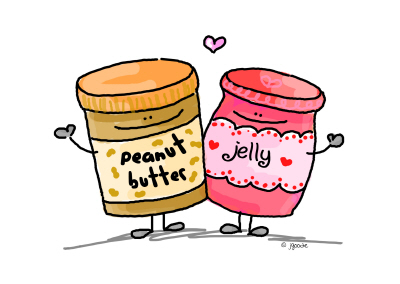
\includegraphics[width=0.6\textwidth]{figures/peanutbutterlover}}
\only<2>{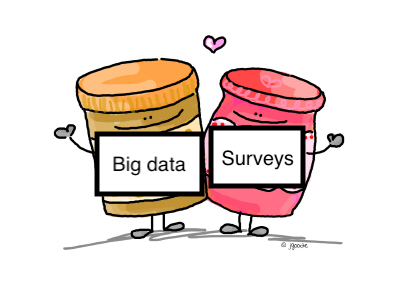
\includegraphics[width=0.6\textwidth]{figures/peanutbutterlover_bigdata_survey}}
\end{center}

\vfill
\tiny{\url{http://schlitterblog.com/wp-content/uploads/2014/05/peanutbutterlover.jpg}}

\end{frame}
%%%%%%%%%%%%%%%%%%%%%%%%%%%
\begin{frame}

\begin{center}
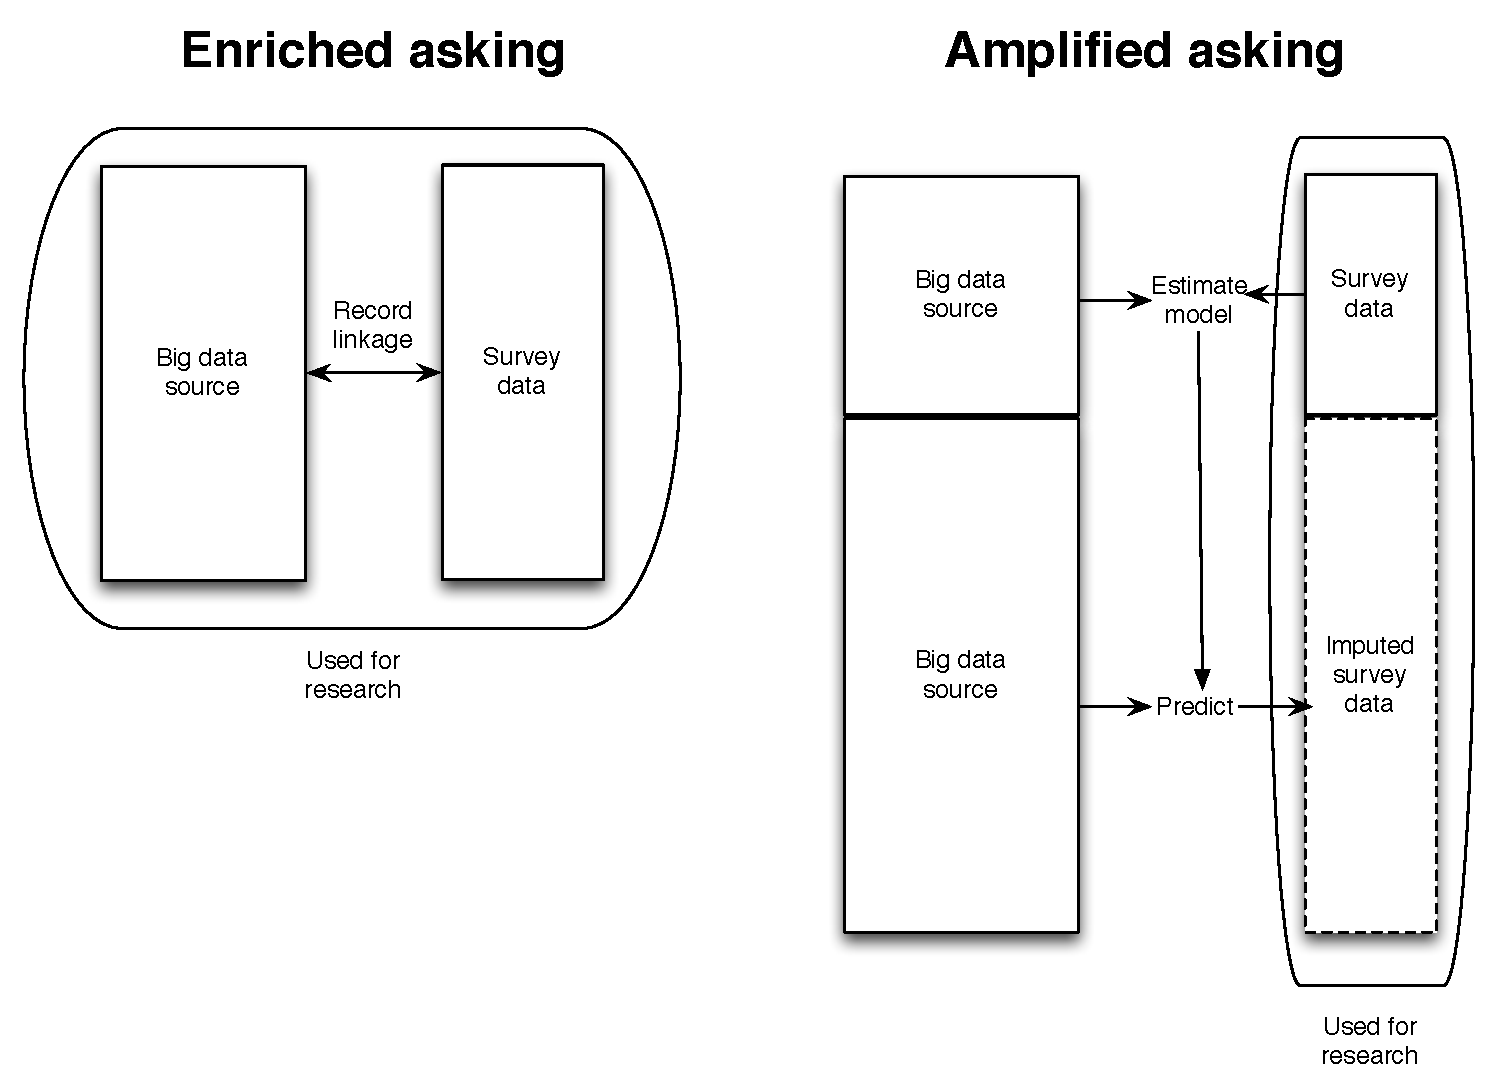
\includegraphics[width=0.6\textwidth]{figures/bitbybit3-12_found_survey_combined}
\end{center}

Note the different role of the big data in each case

\end{frame}
%%%%%%%%%%%%%%%%%%%%%%%%%%%
\begin{frame}

\begin{center}

\includegraphics[width=0.6\textwidth]{figures/ansolabehere_validation_2012_title}
\end{center}

\vfill
\href{https://www.jstor.org/stable/23359641}{Ansolabehere and Hersh (2012)}
\end{frame}
%%%%%%%%%%%%%%%%%%%%%%%%%%%
\begin{frame}

\begin{center}
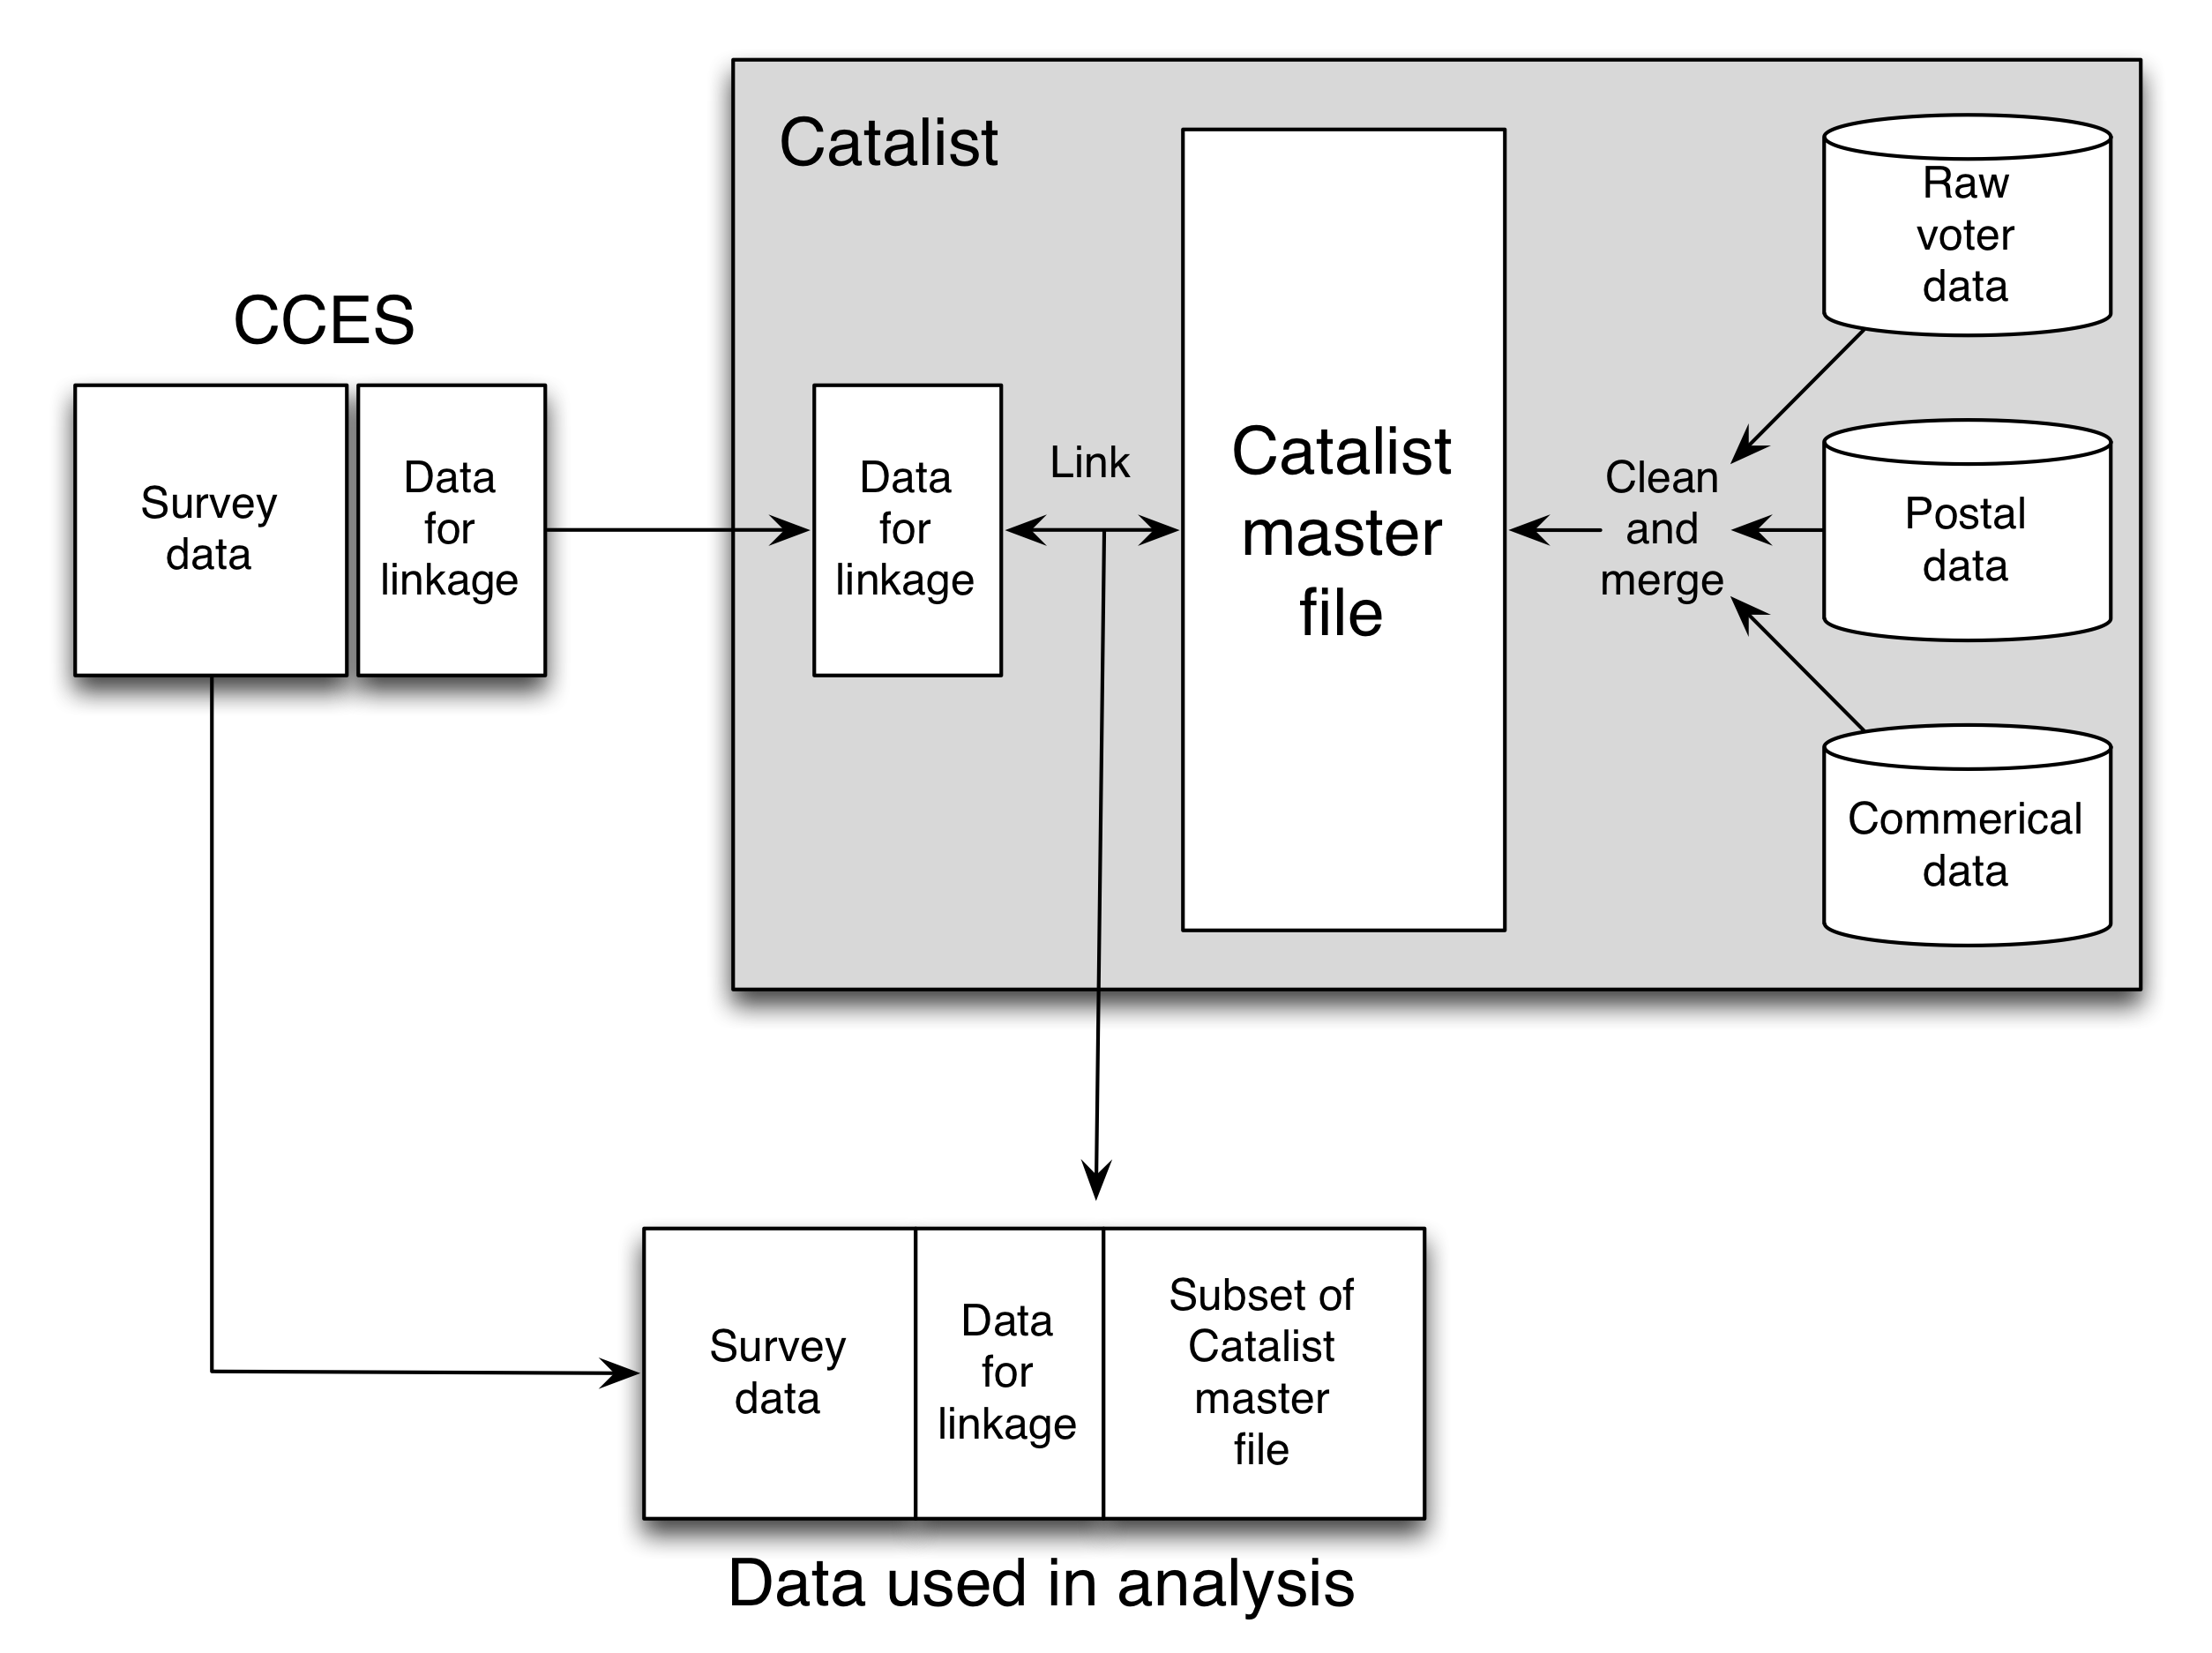
\includegraphics[width=0.6\textwidth]{figures/bitbybit3-13_ansolabehere_validation_2012_schematic}
\end{center}

\vfill
\href{https://www.jstor.org/stable/23359641}{Ansolabehere and Hersh (2012)}
\end{frame}
%%%%%%%%%%%%%%%%%%%%%%%%%%%
\begin{frame}

\begin{center}
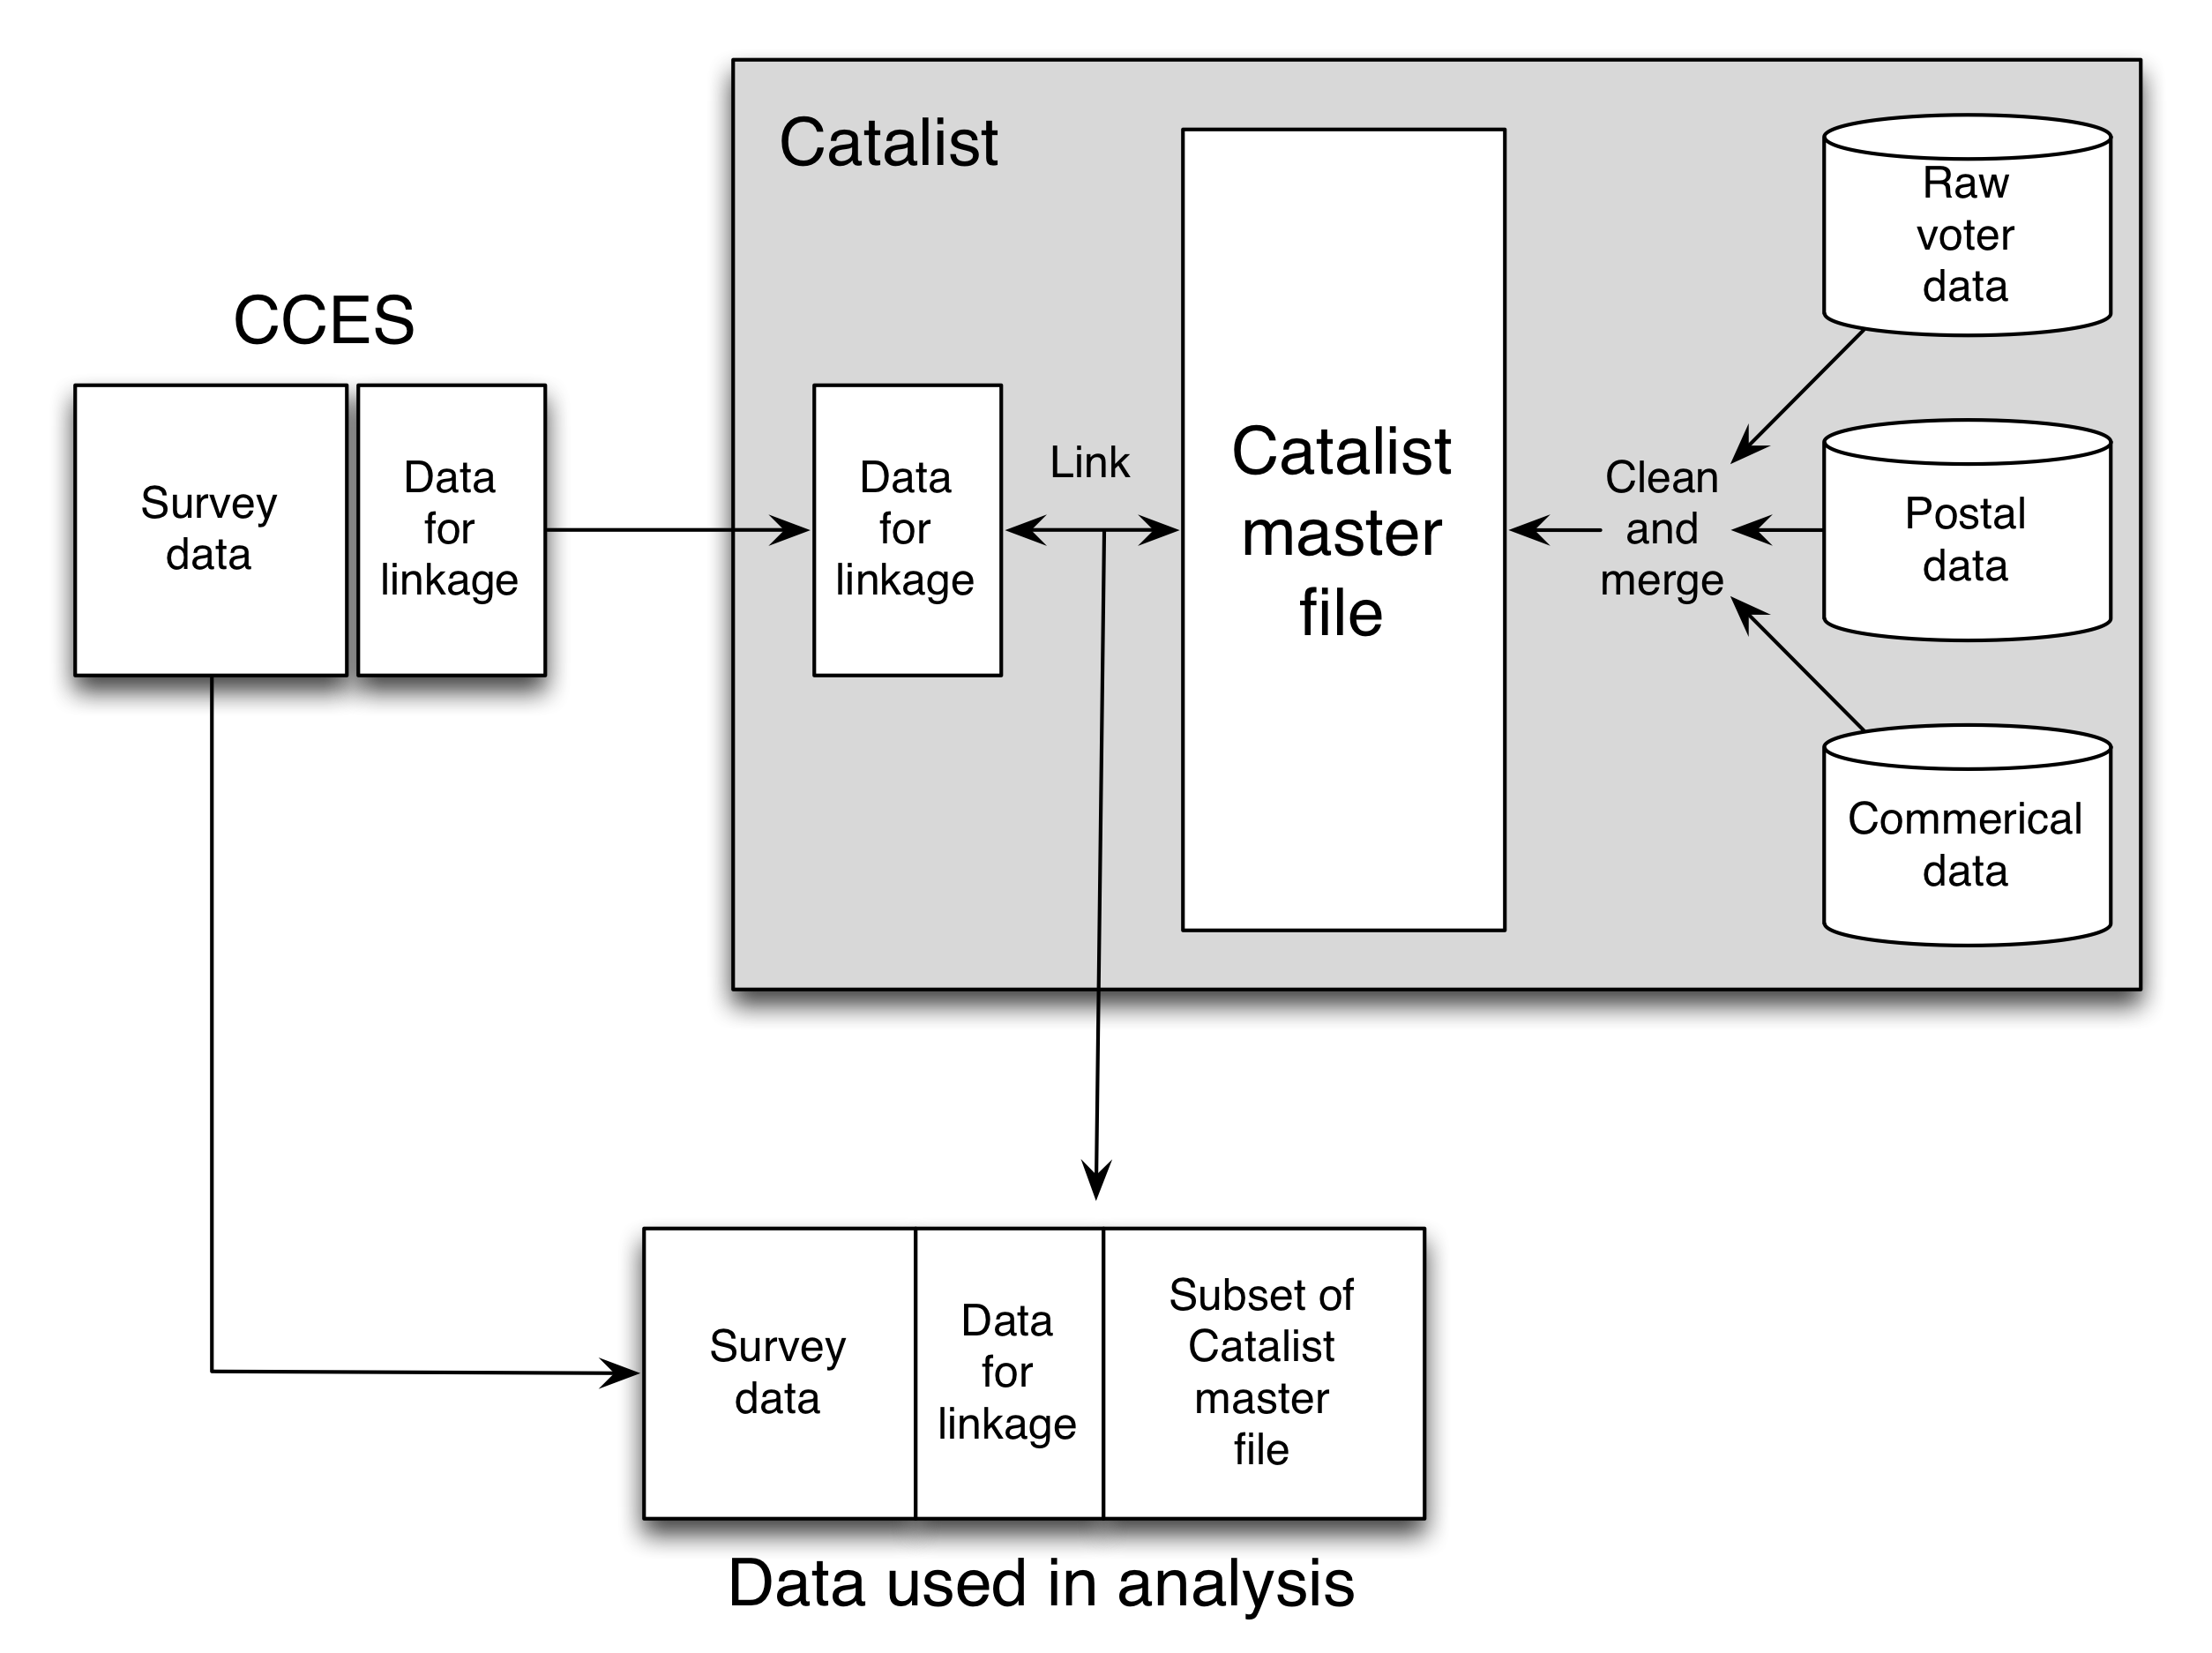
\includegraphics[width=0.2\textwidth]{figures/bitbybit3-13_ansolabehere_validation_2012_schematic}
\end{center}
Findings:
\begin{itemize}
\item Over-reporting of voting is rampant: almost half of non-voters reported voting, someone who reported voting had 80\% chance of actually voting
\pause
\item Over-reporting is not random; it is more common among high-income, well-educated, partisans engaged in civic affairs
\pause
\item Because of systematic over-reporting, differences between voters and nonvoters are smaller than they appear from surveys
\pause
\item Existing theories are better at predicting who will reporting voting than who will actually vote
\end{itemize}
\vfill
\href{https://www.jstor.org/stable/23359641}{Ansolabehere and Hersh (2012)}
\end{frame}
%%%%%%%%%%%%%%%%%%%%%%%%%%%
\begin{frame}

\begin{center}
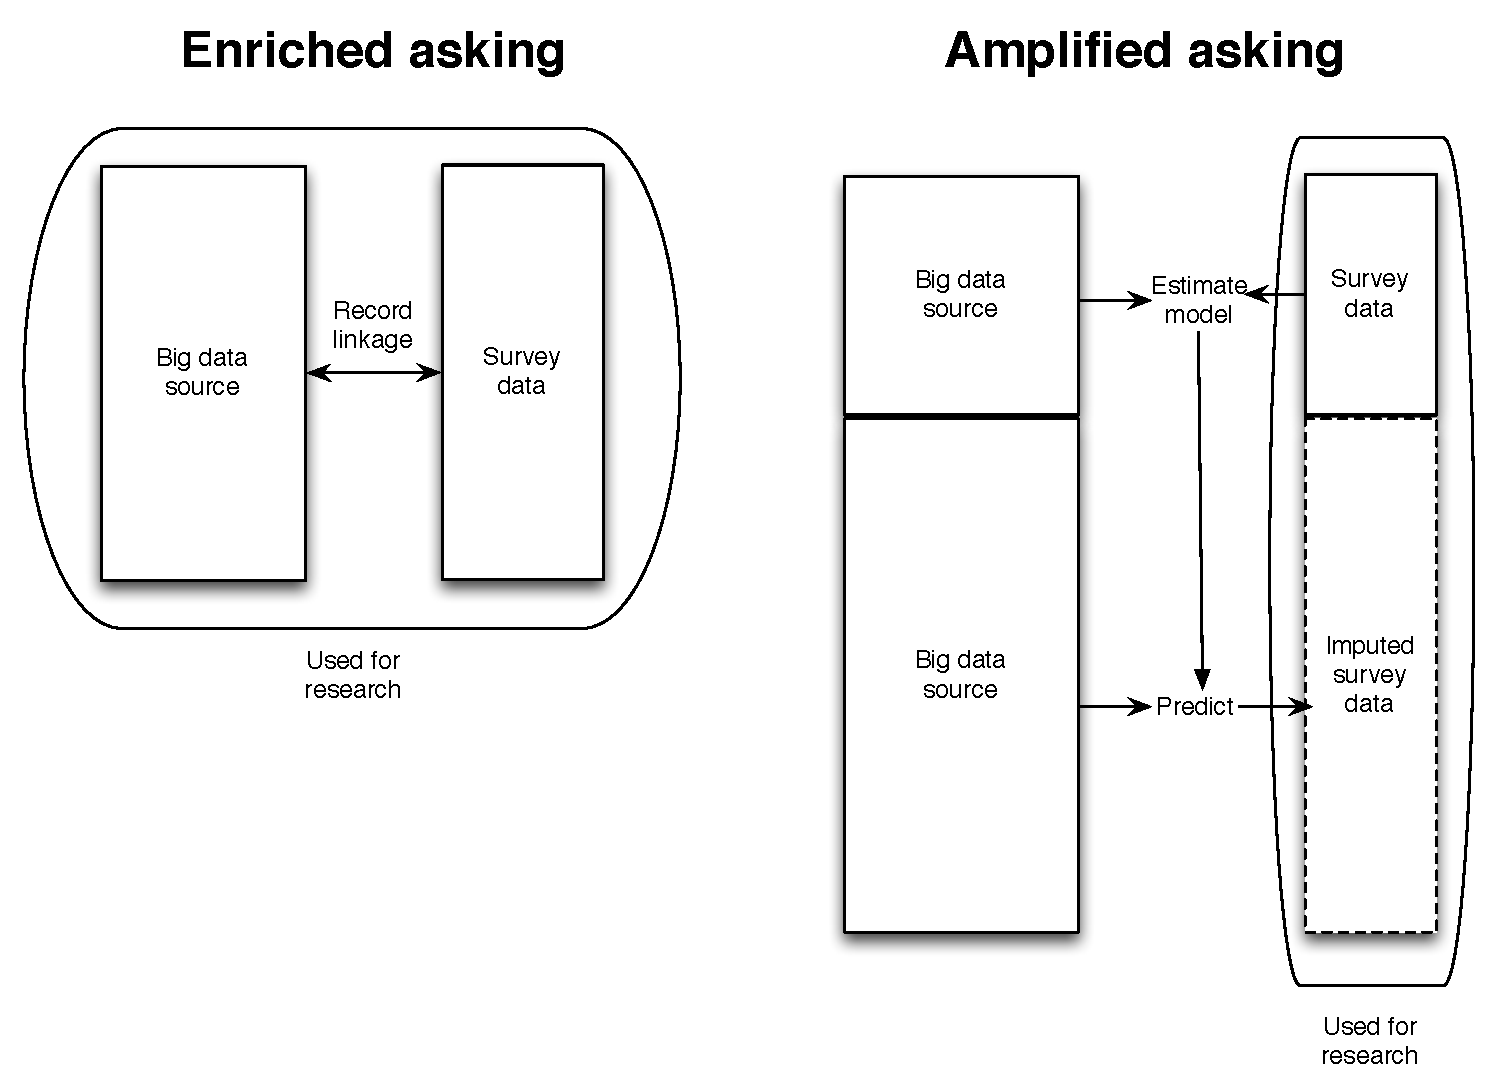
\includegraphics[width=0.6\textwidth]{figures/bitbybit3-12_found_survey_combined}
\end{center}

Note the different role of the big data in each case

\end{frame}
%%%%%%%%%%%%%%%%%%%%%%%%%%%
\begin{frame}

\begin{center}
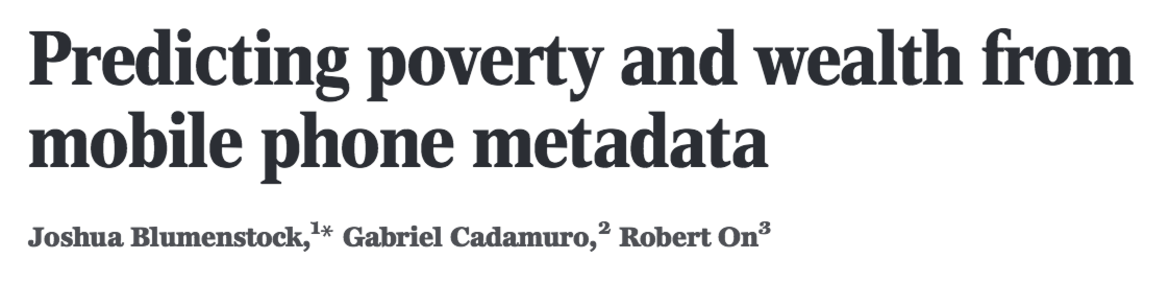
\includegraphics[width=0.6\textwidth]{figures/blumenstock_predicting_2015_title}
\end{center}

\vfill
\href{https://dx.doi/10.1126/science.aac4420}{Blumenstock, Cadamuro, and On (2015)}
\end{frame}
%%%%%%%%%%%%%%%%%%%%%%%%%%%
\begin{frame}

\begin{center}
\only<1>{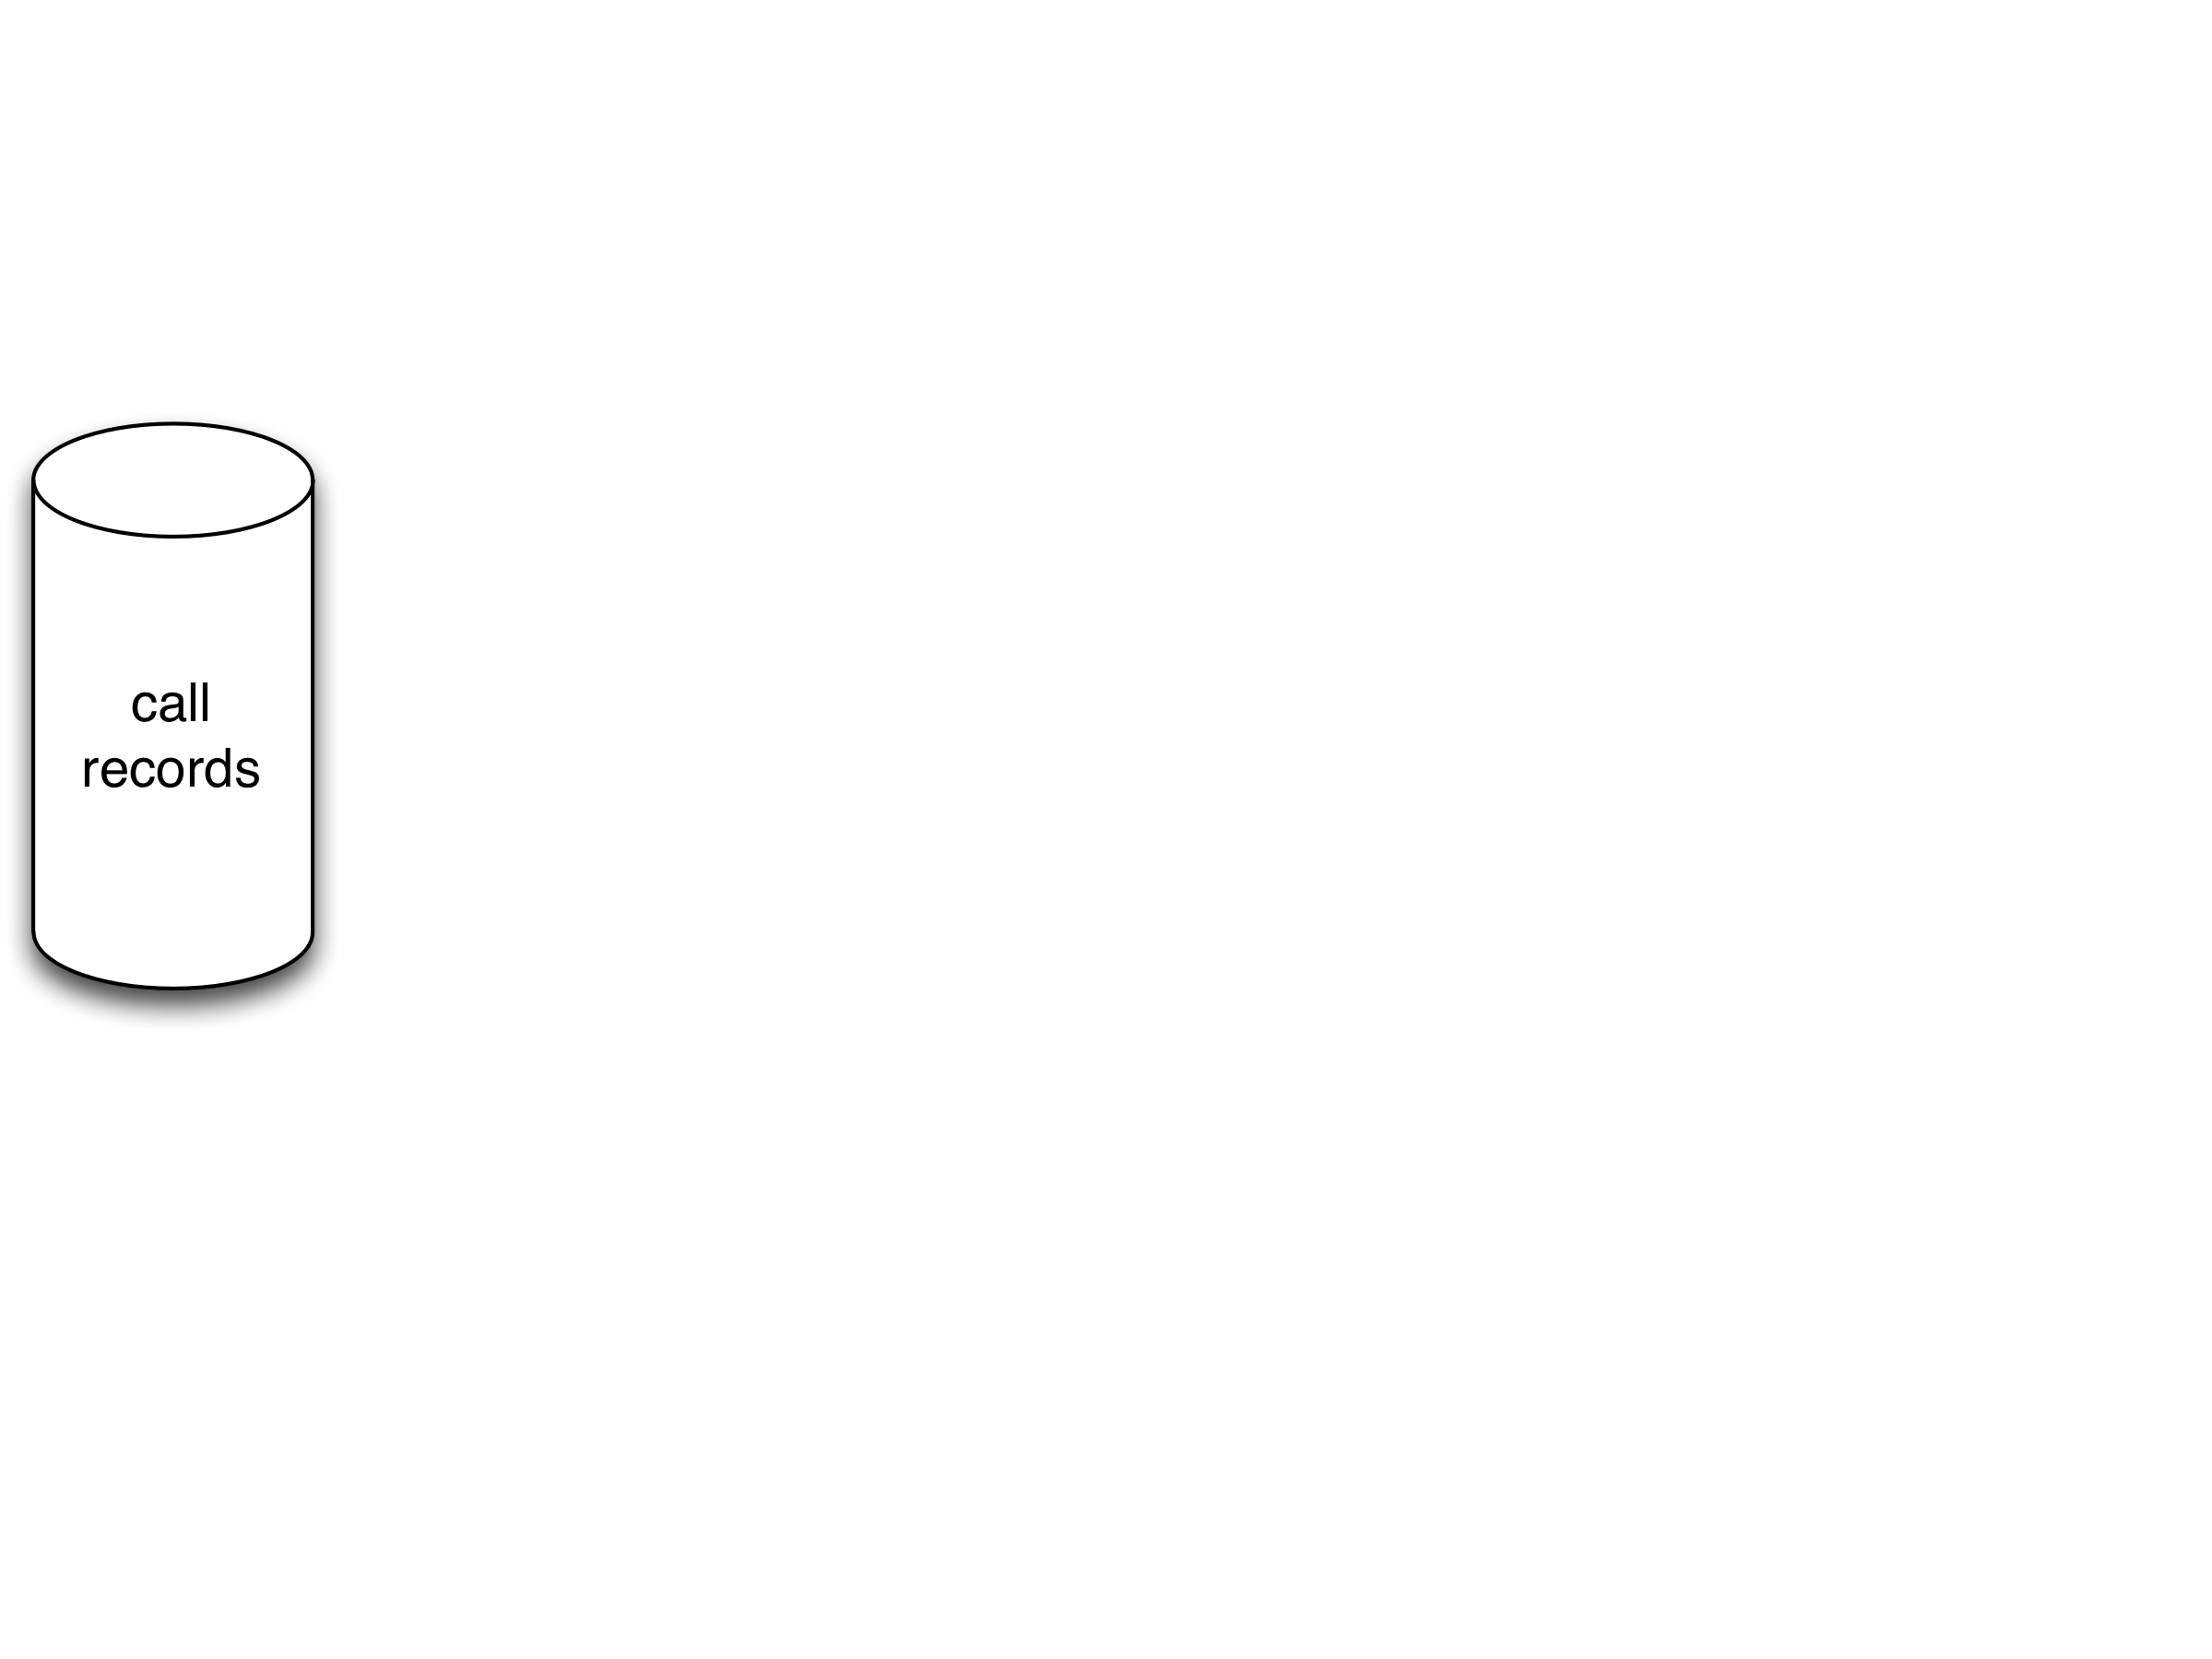
\includegraphics[width=0.7\textwidth]{figures/blumenstock_predicting_2015_schematic_1}}
\only<2>{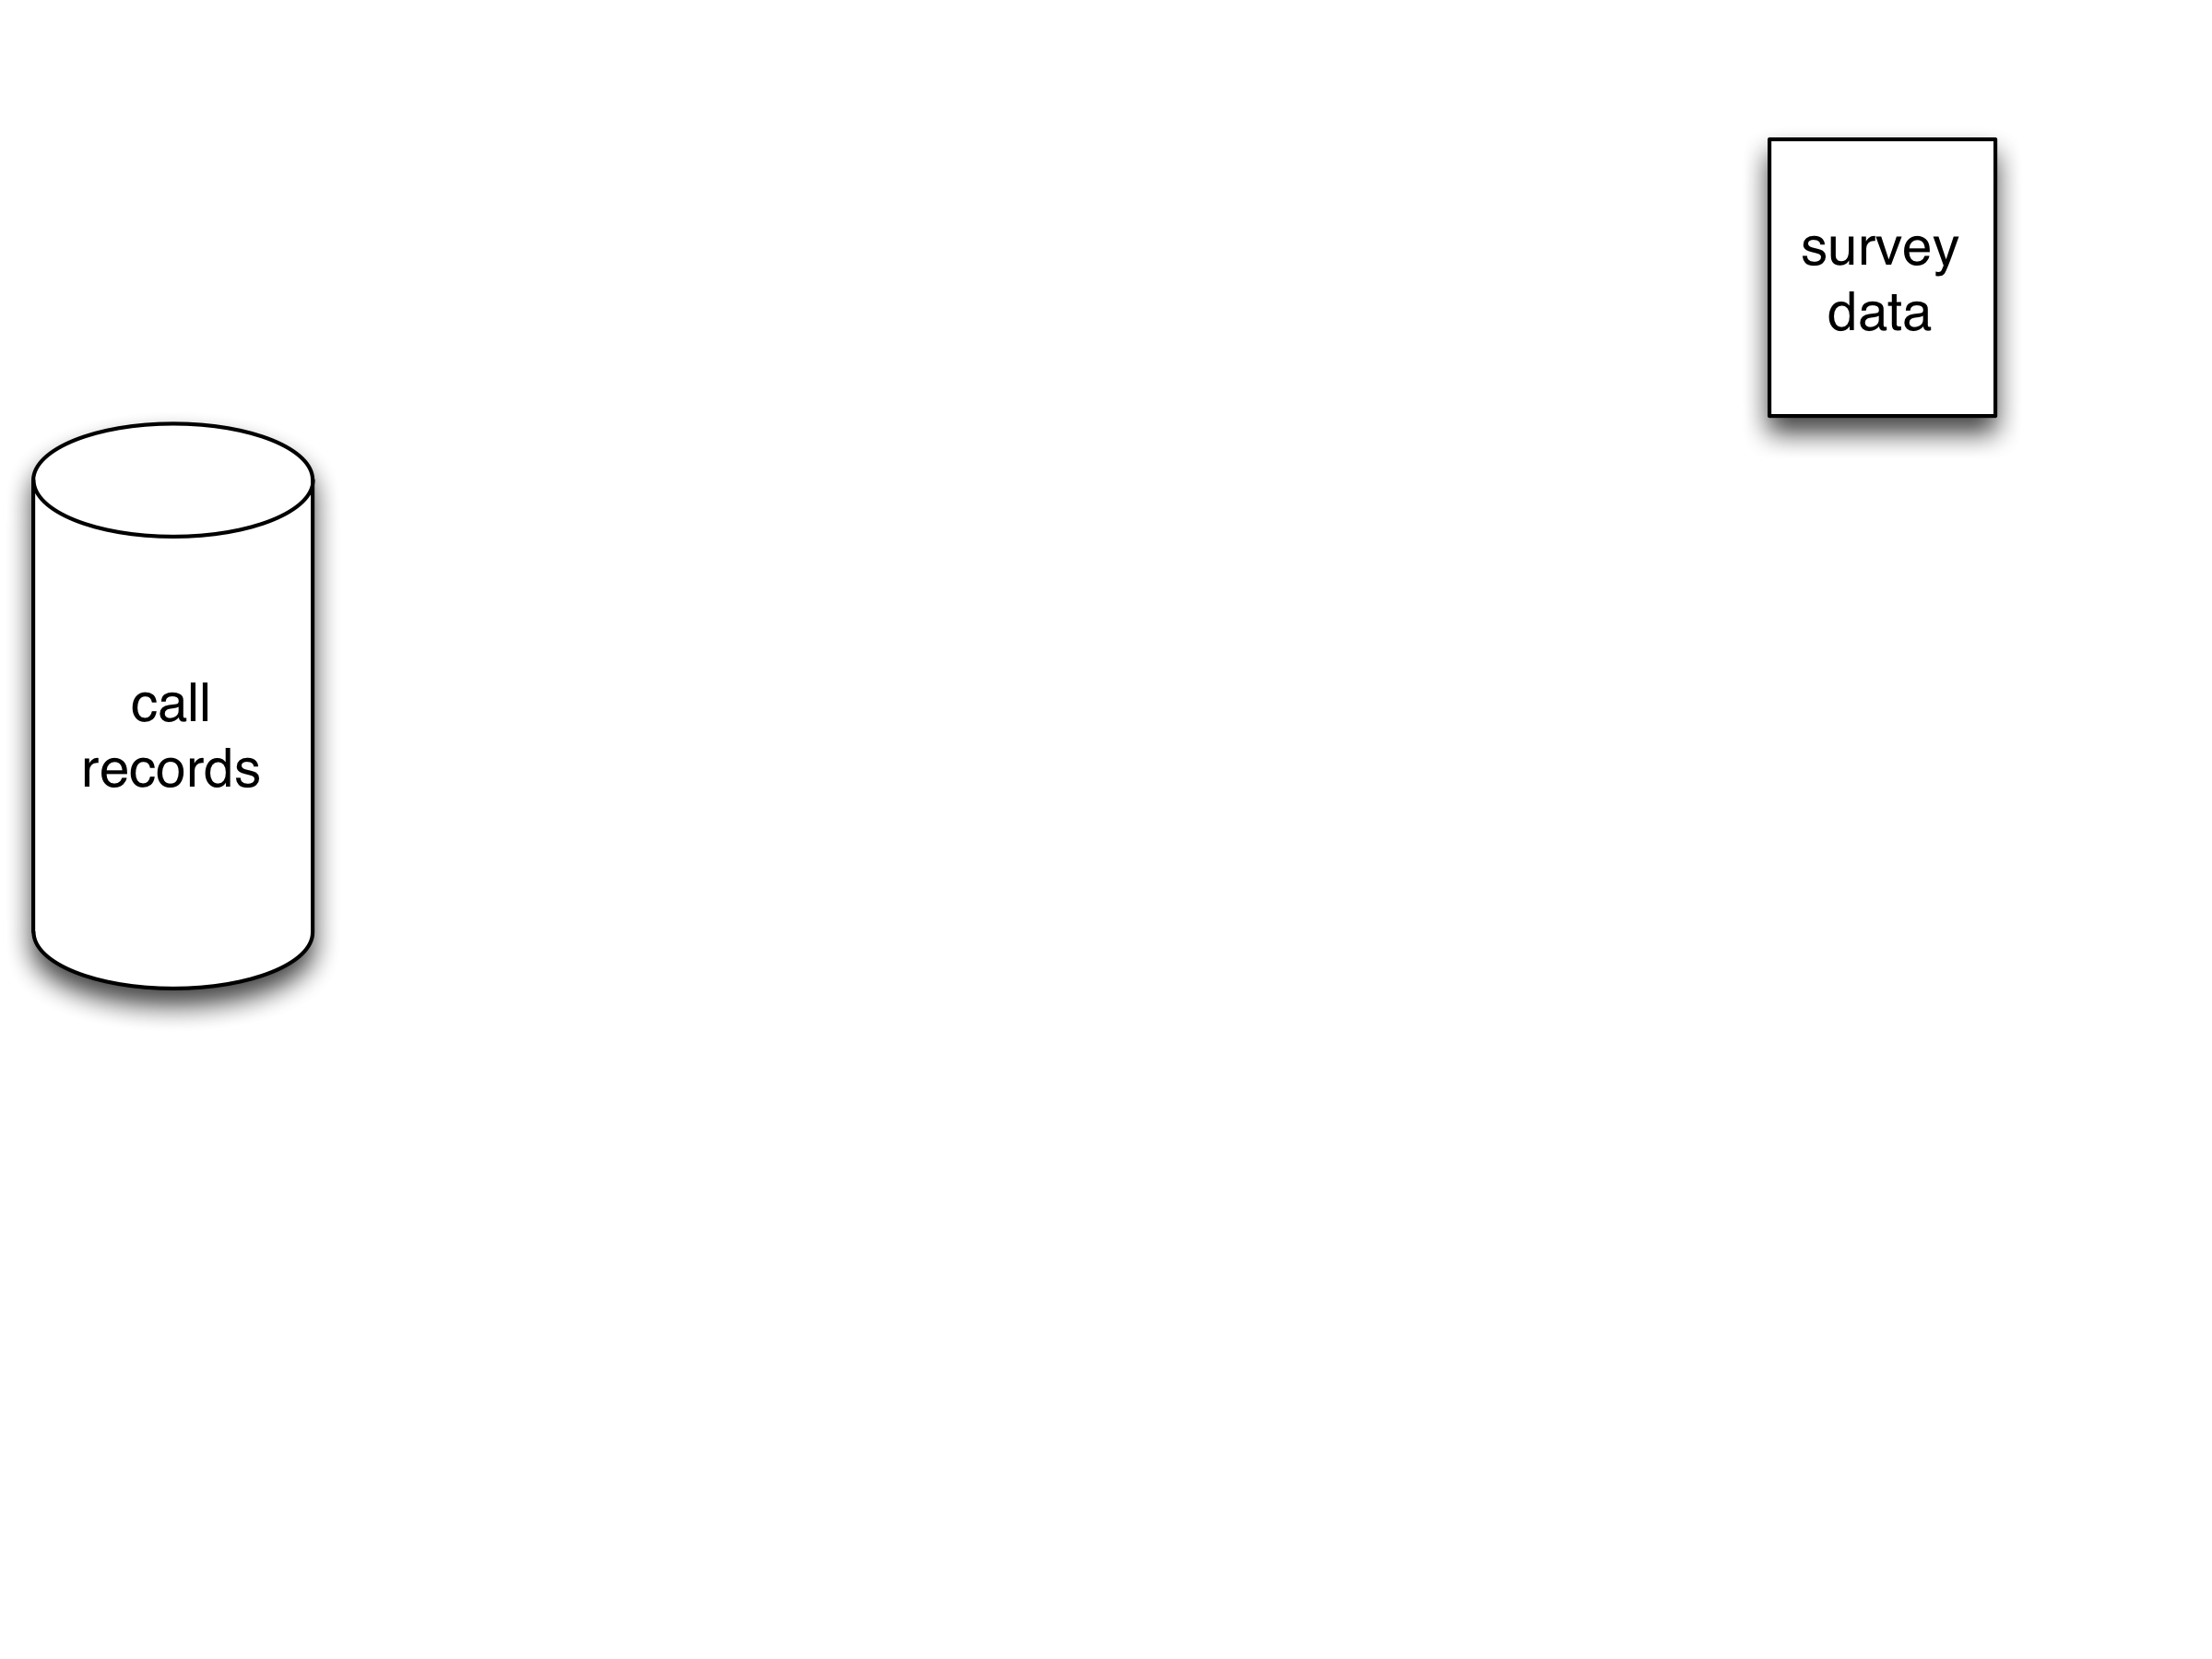
\includegraphics[width=0.7\textwidth]{figures/blumenstock_predicting_2015_schematic_2}}
\only<3>{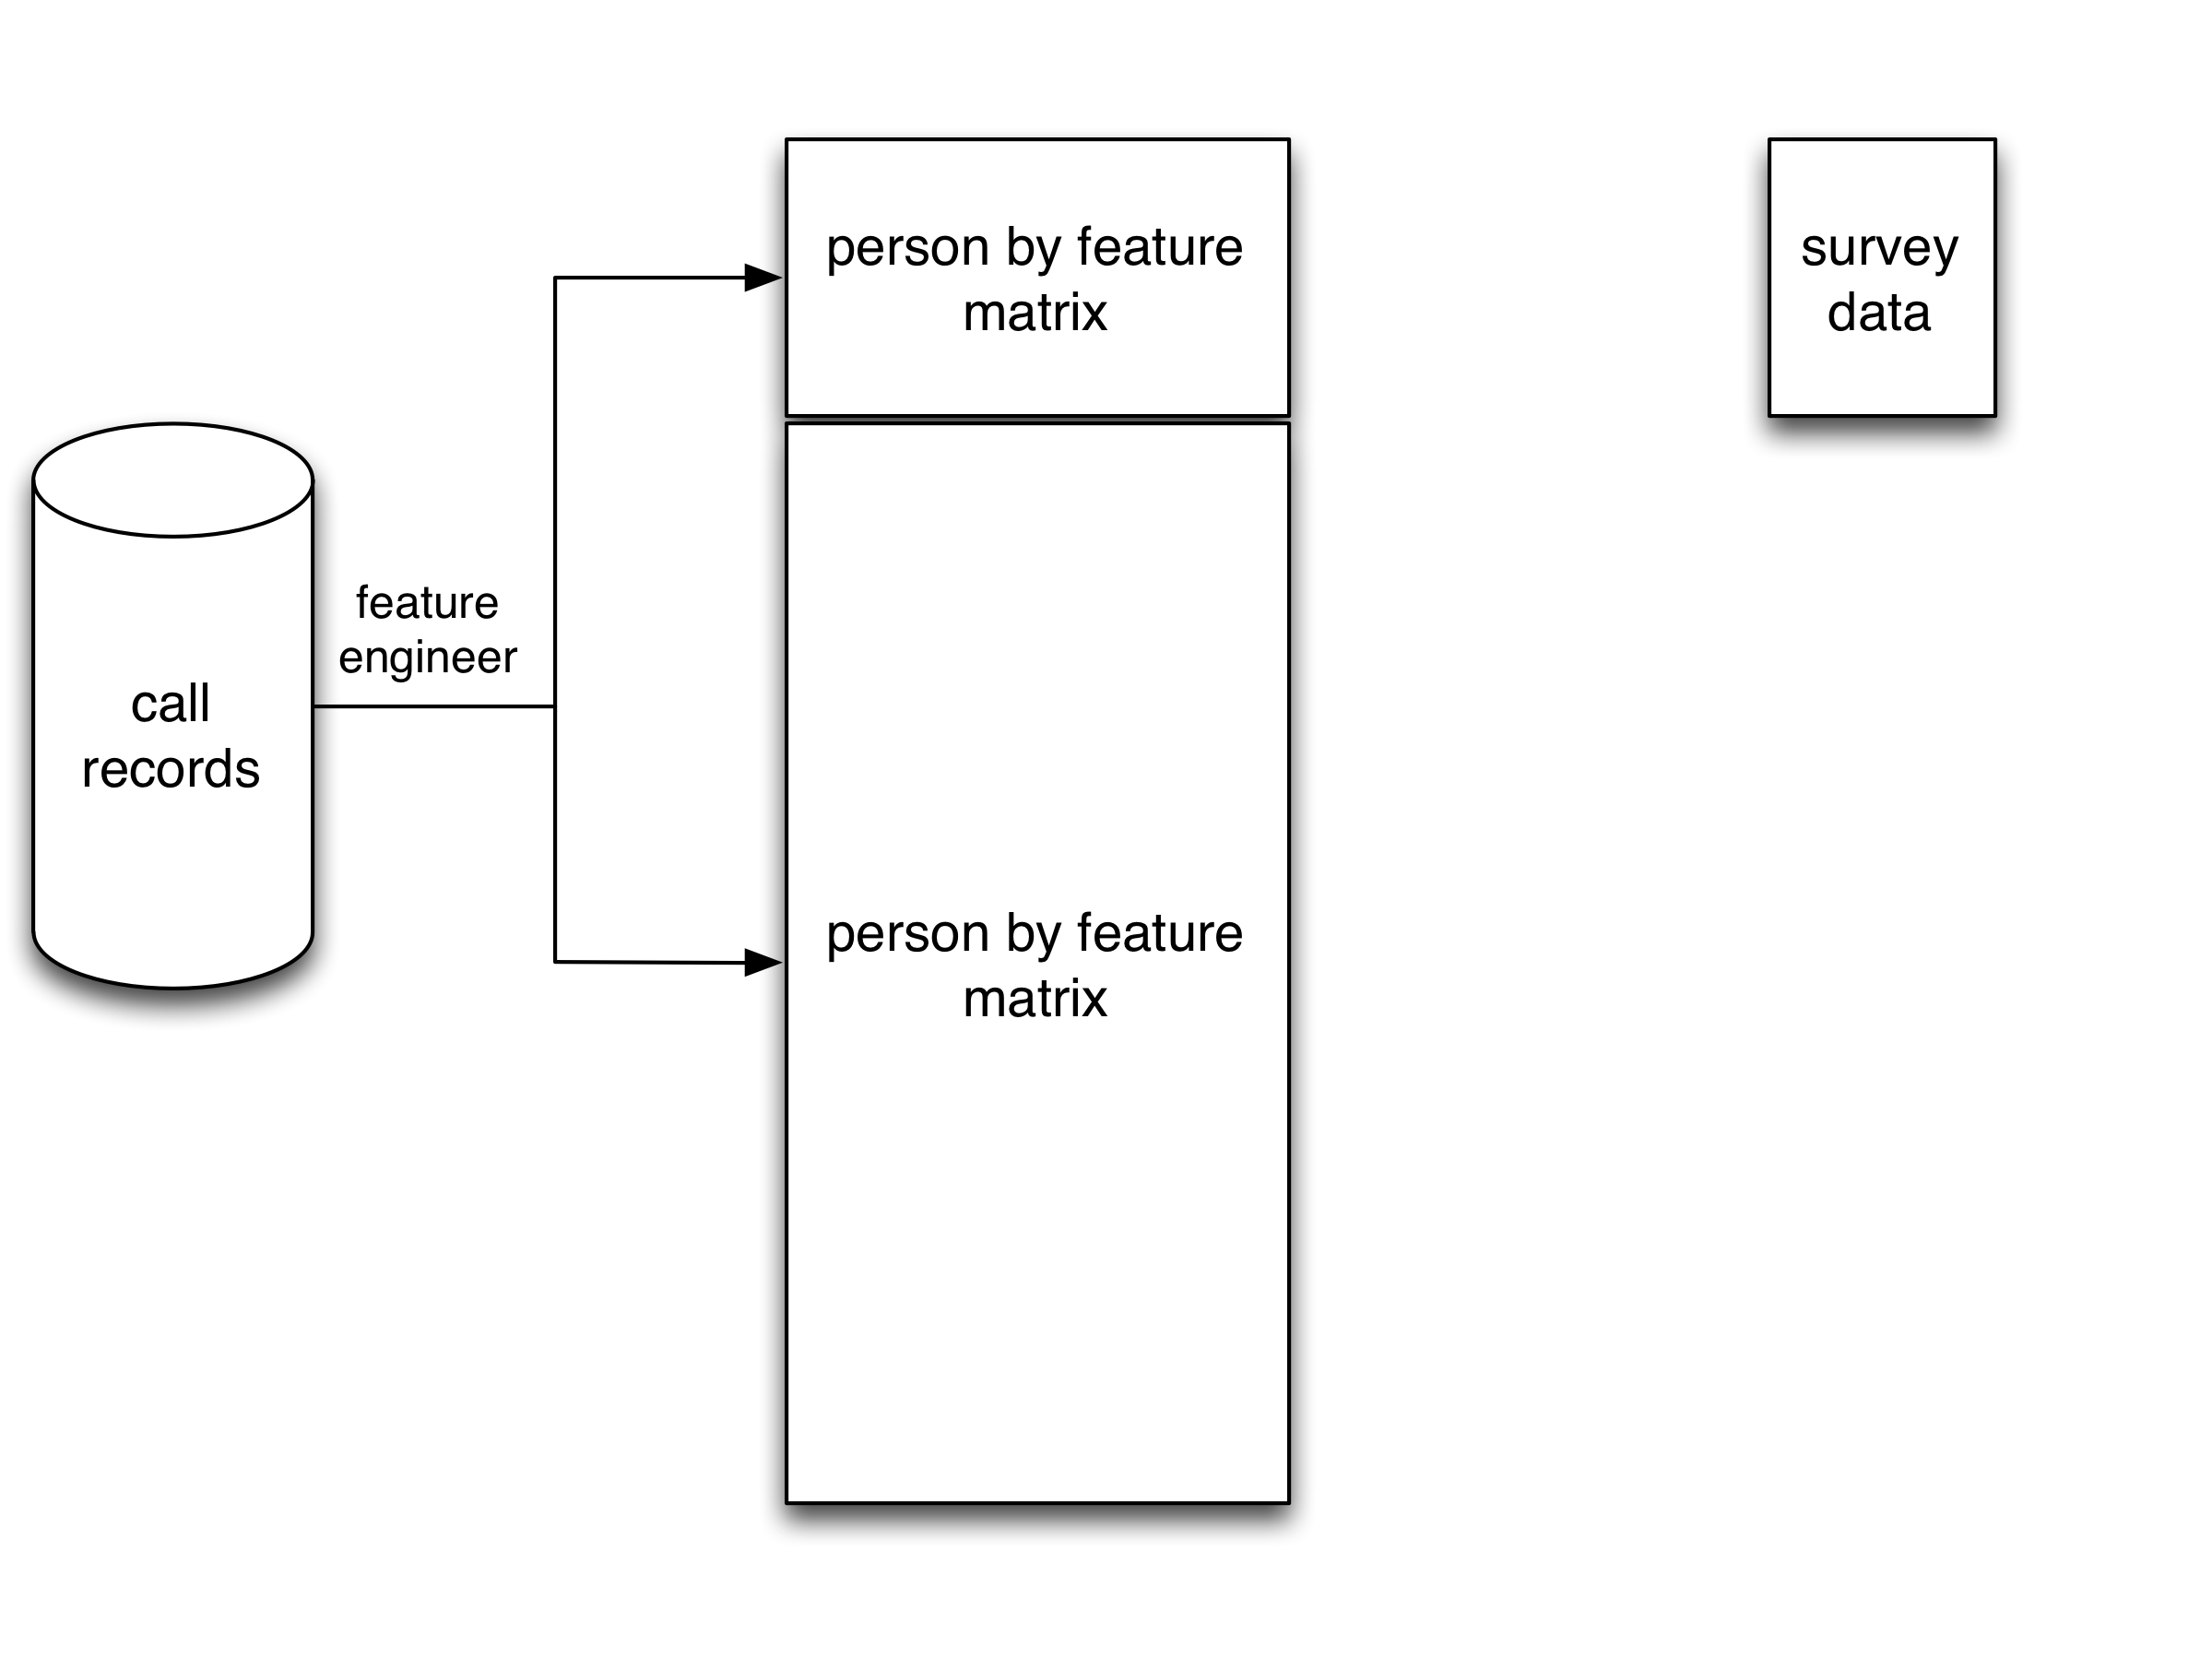
\includegraphics[width=0.7\textwidth]{figures/blumenstock_predicting_2015_schematic_3}}
\only<4>{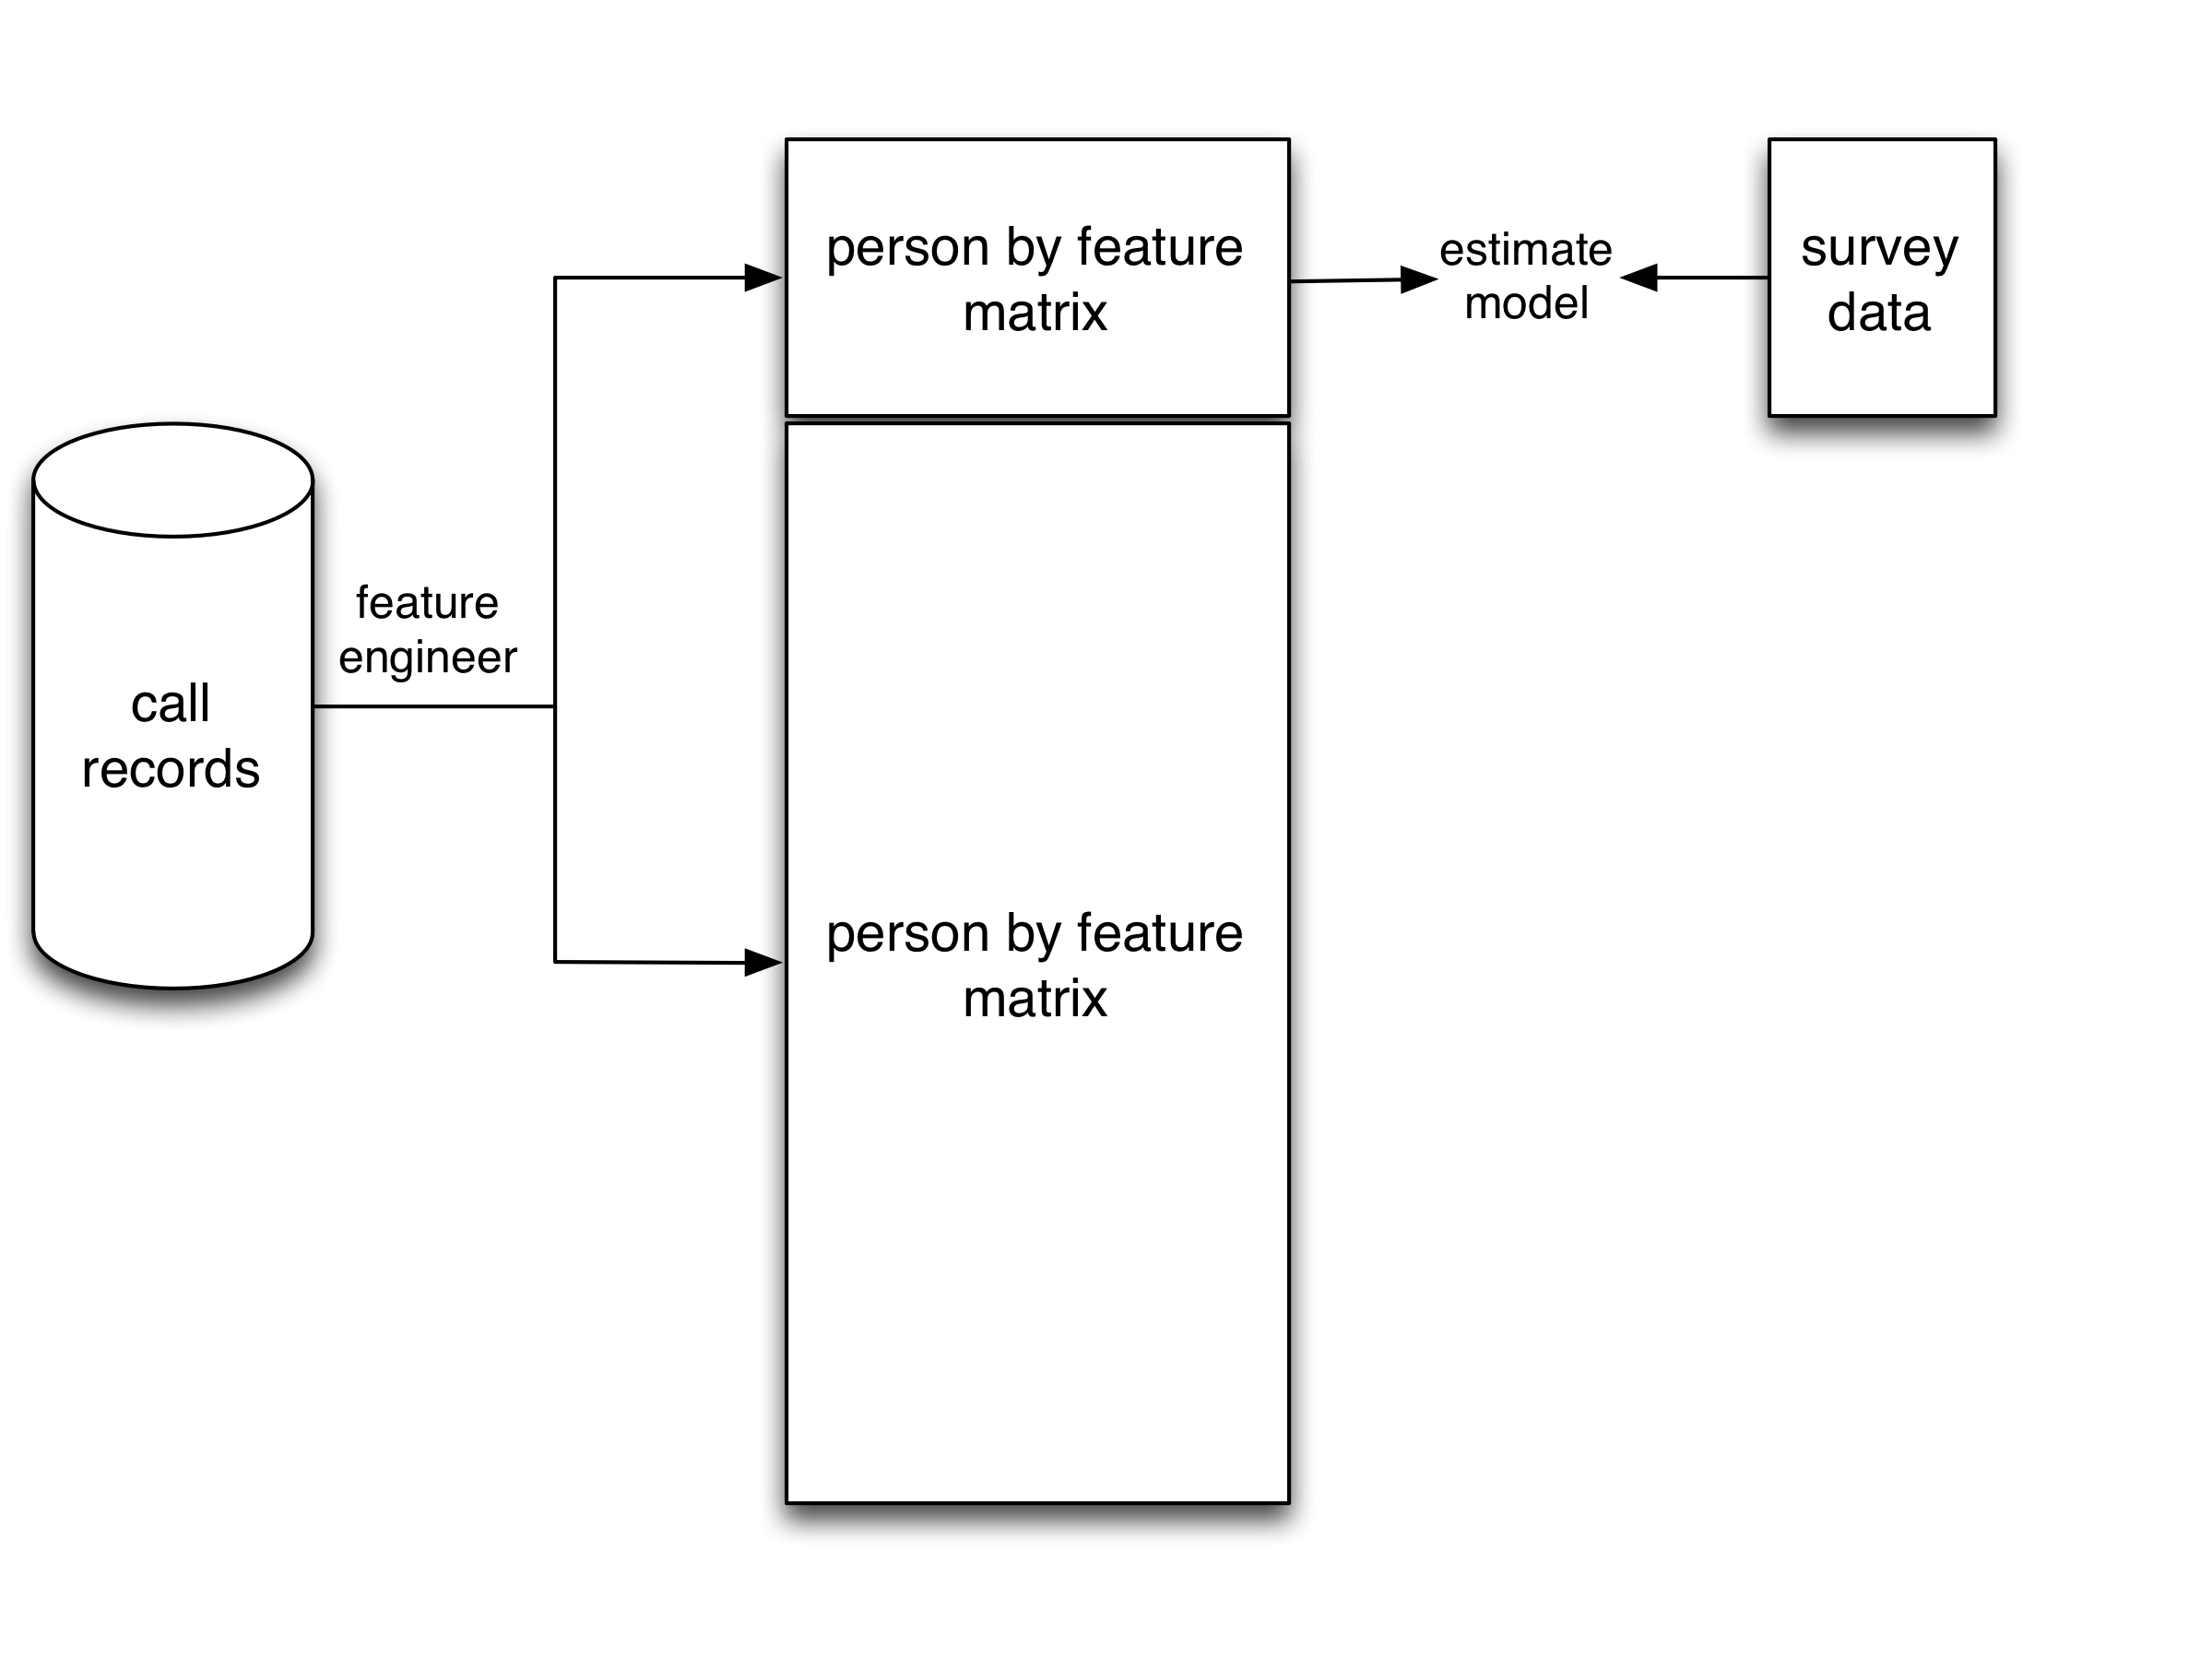
\includegraphics[width=0.7\textwidth]{figures/blumenstock_predicting_2015_schematic_4}}
\only<5>{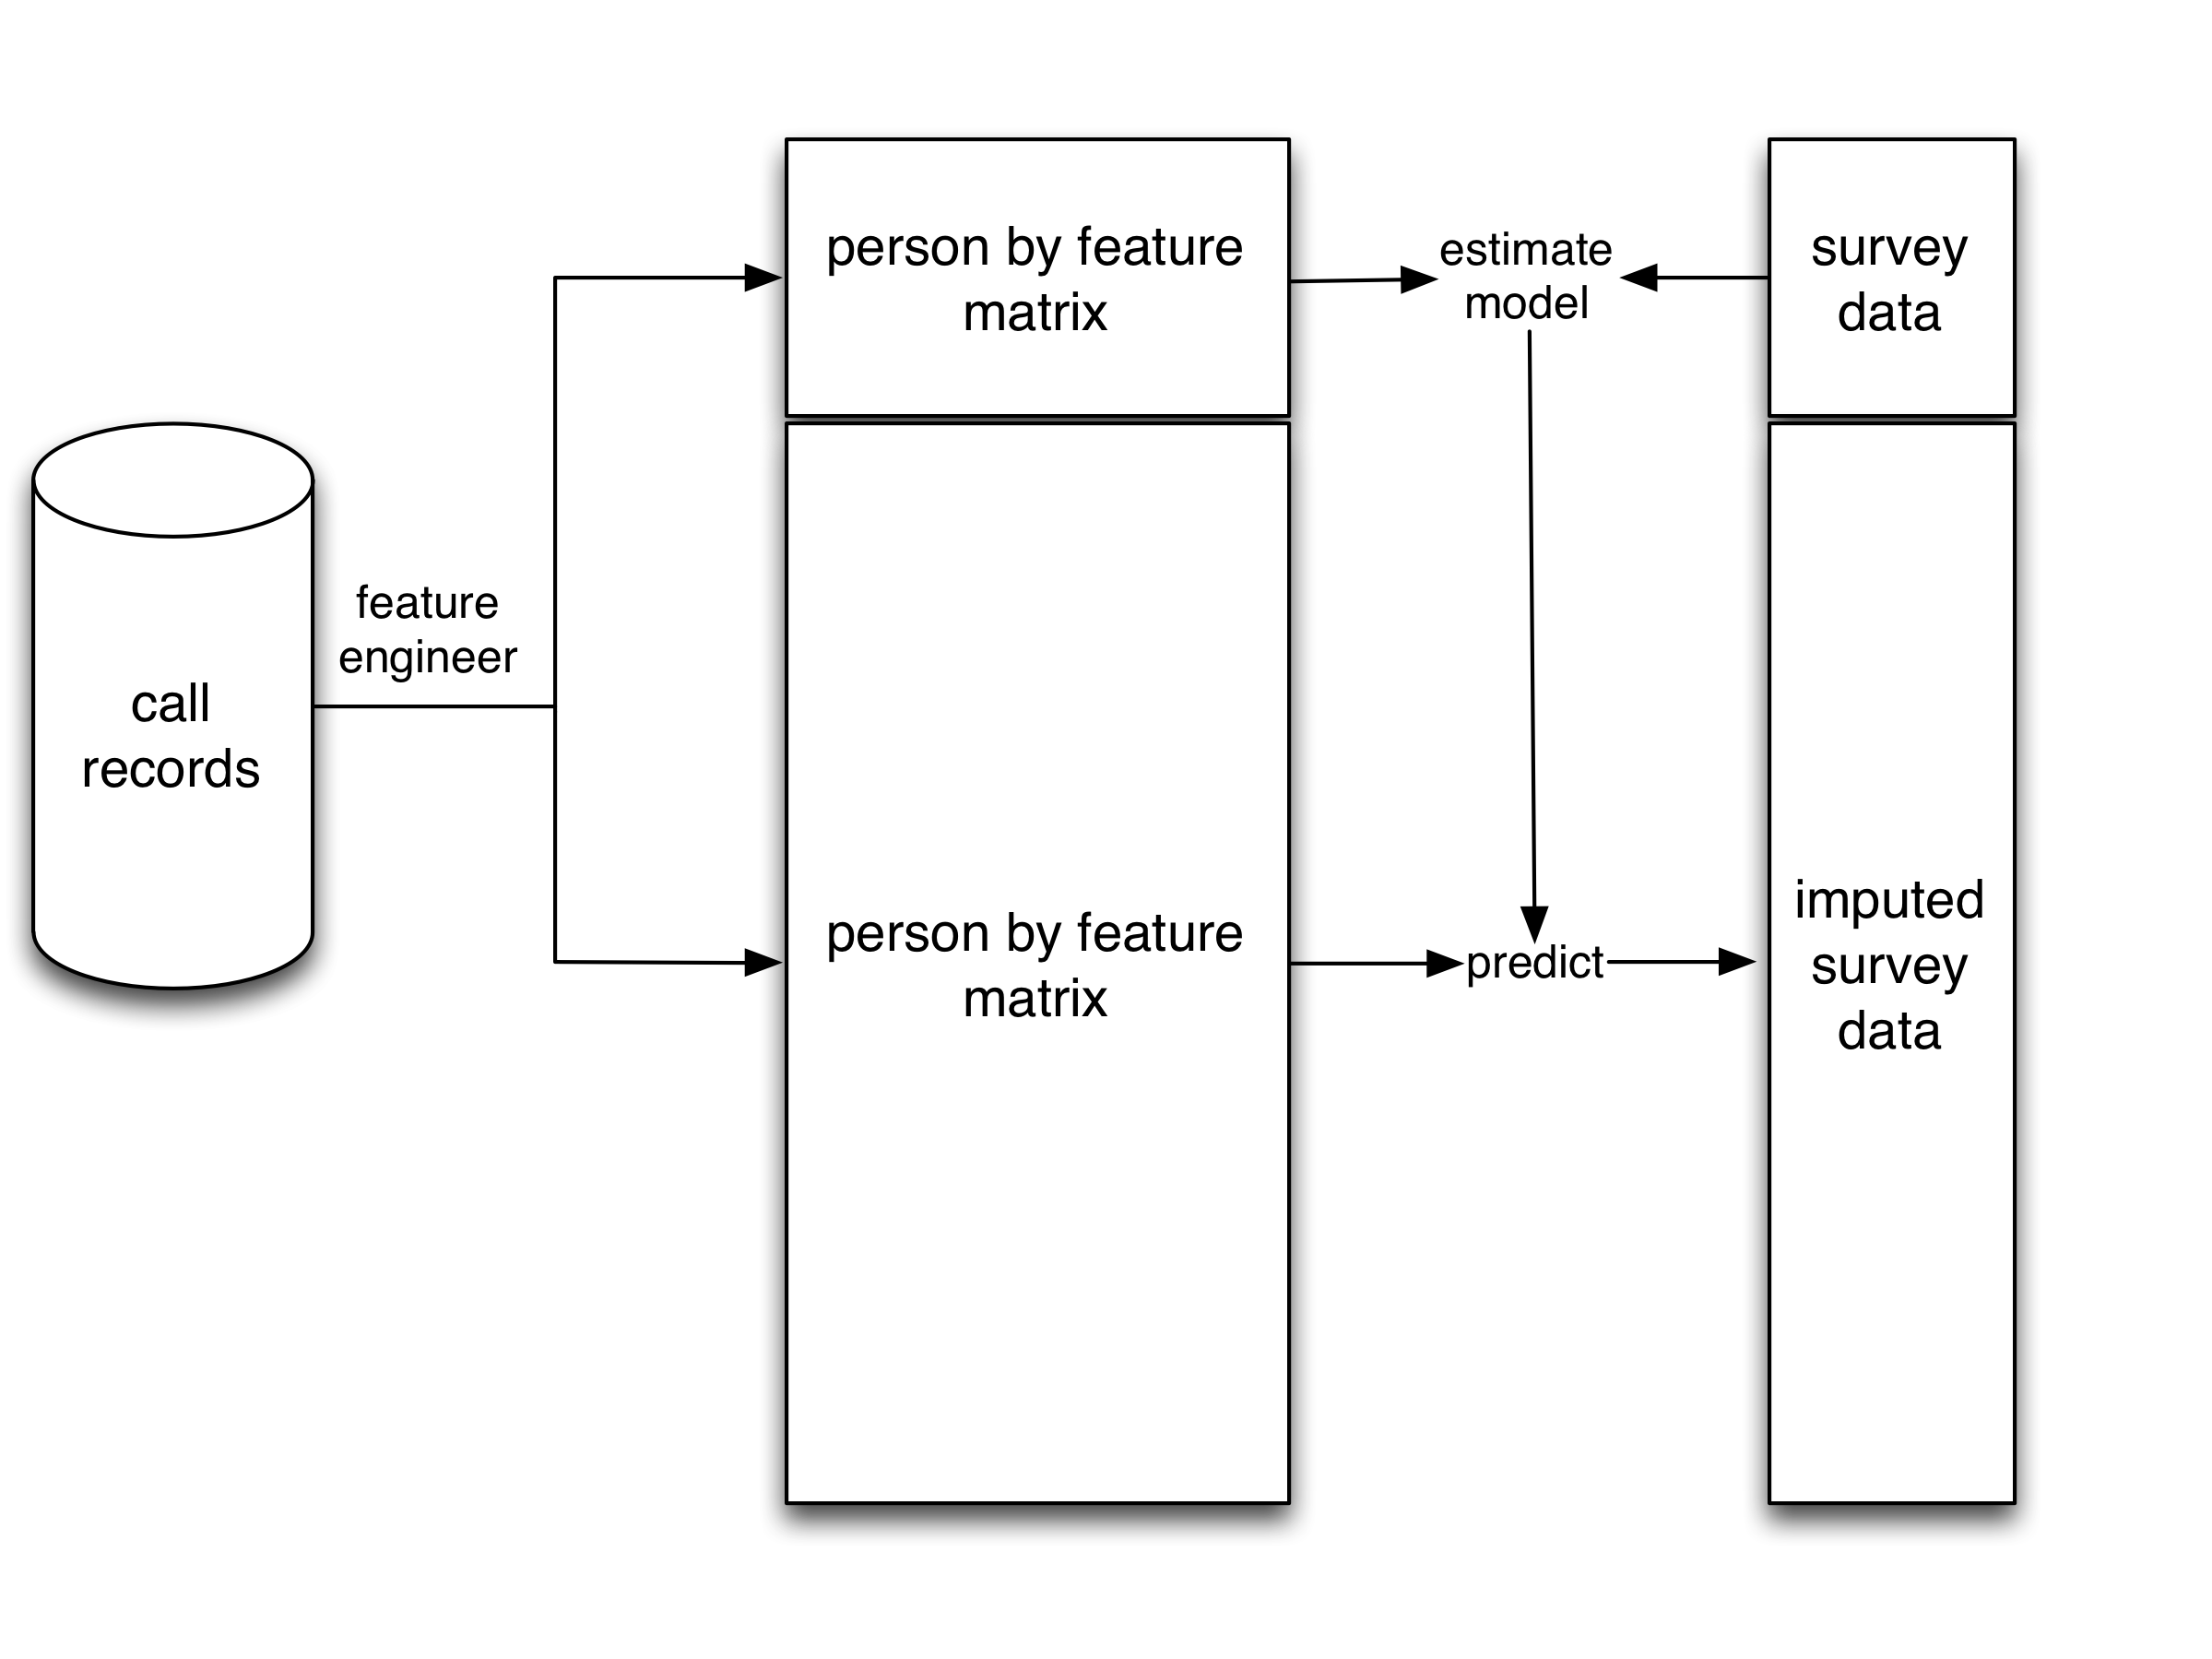
\includegraphics[width=0.7\textwidth]{figures/blumenstock_predicting_2015_schematic_5}}
\only<6>{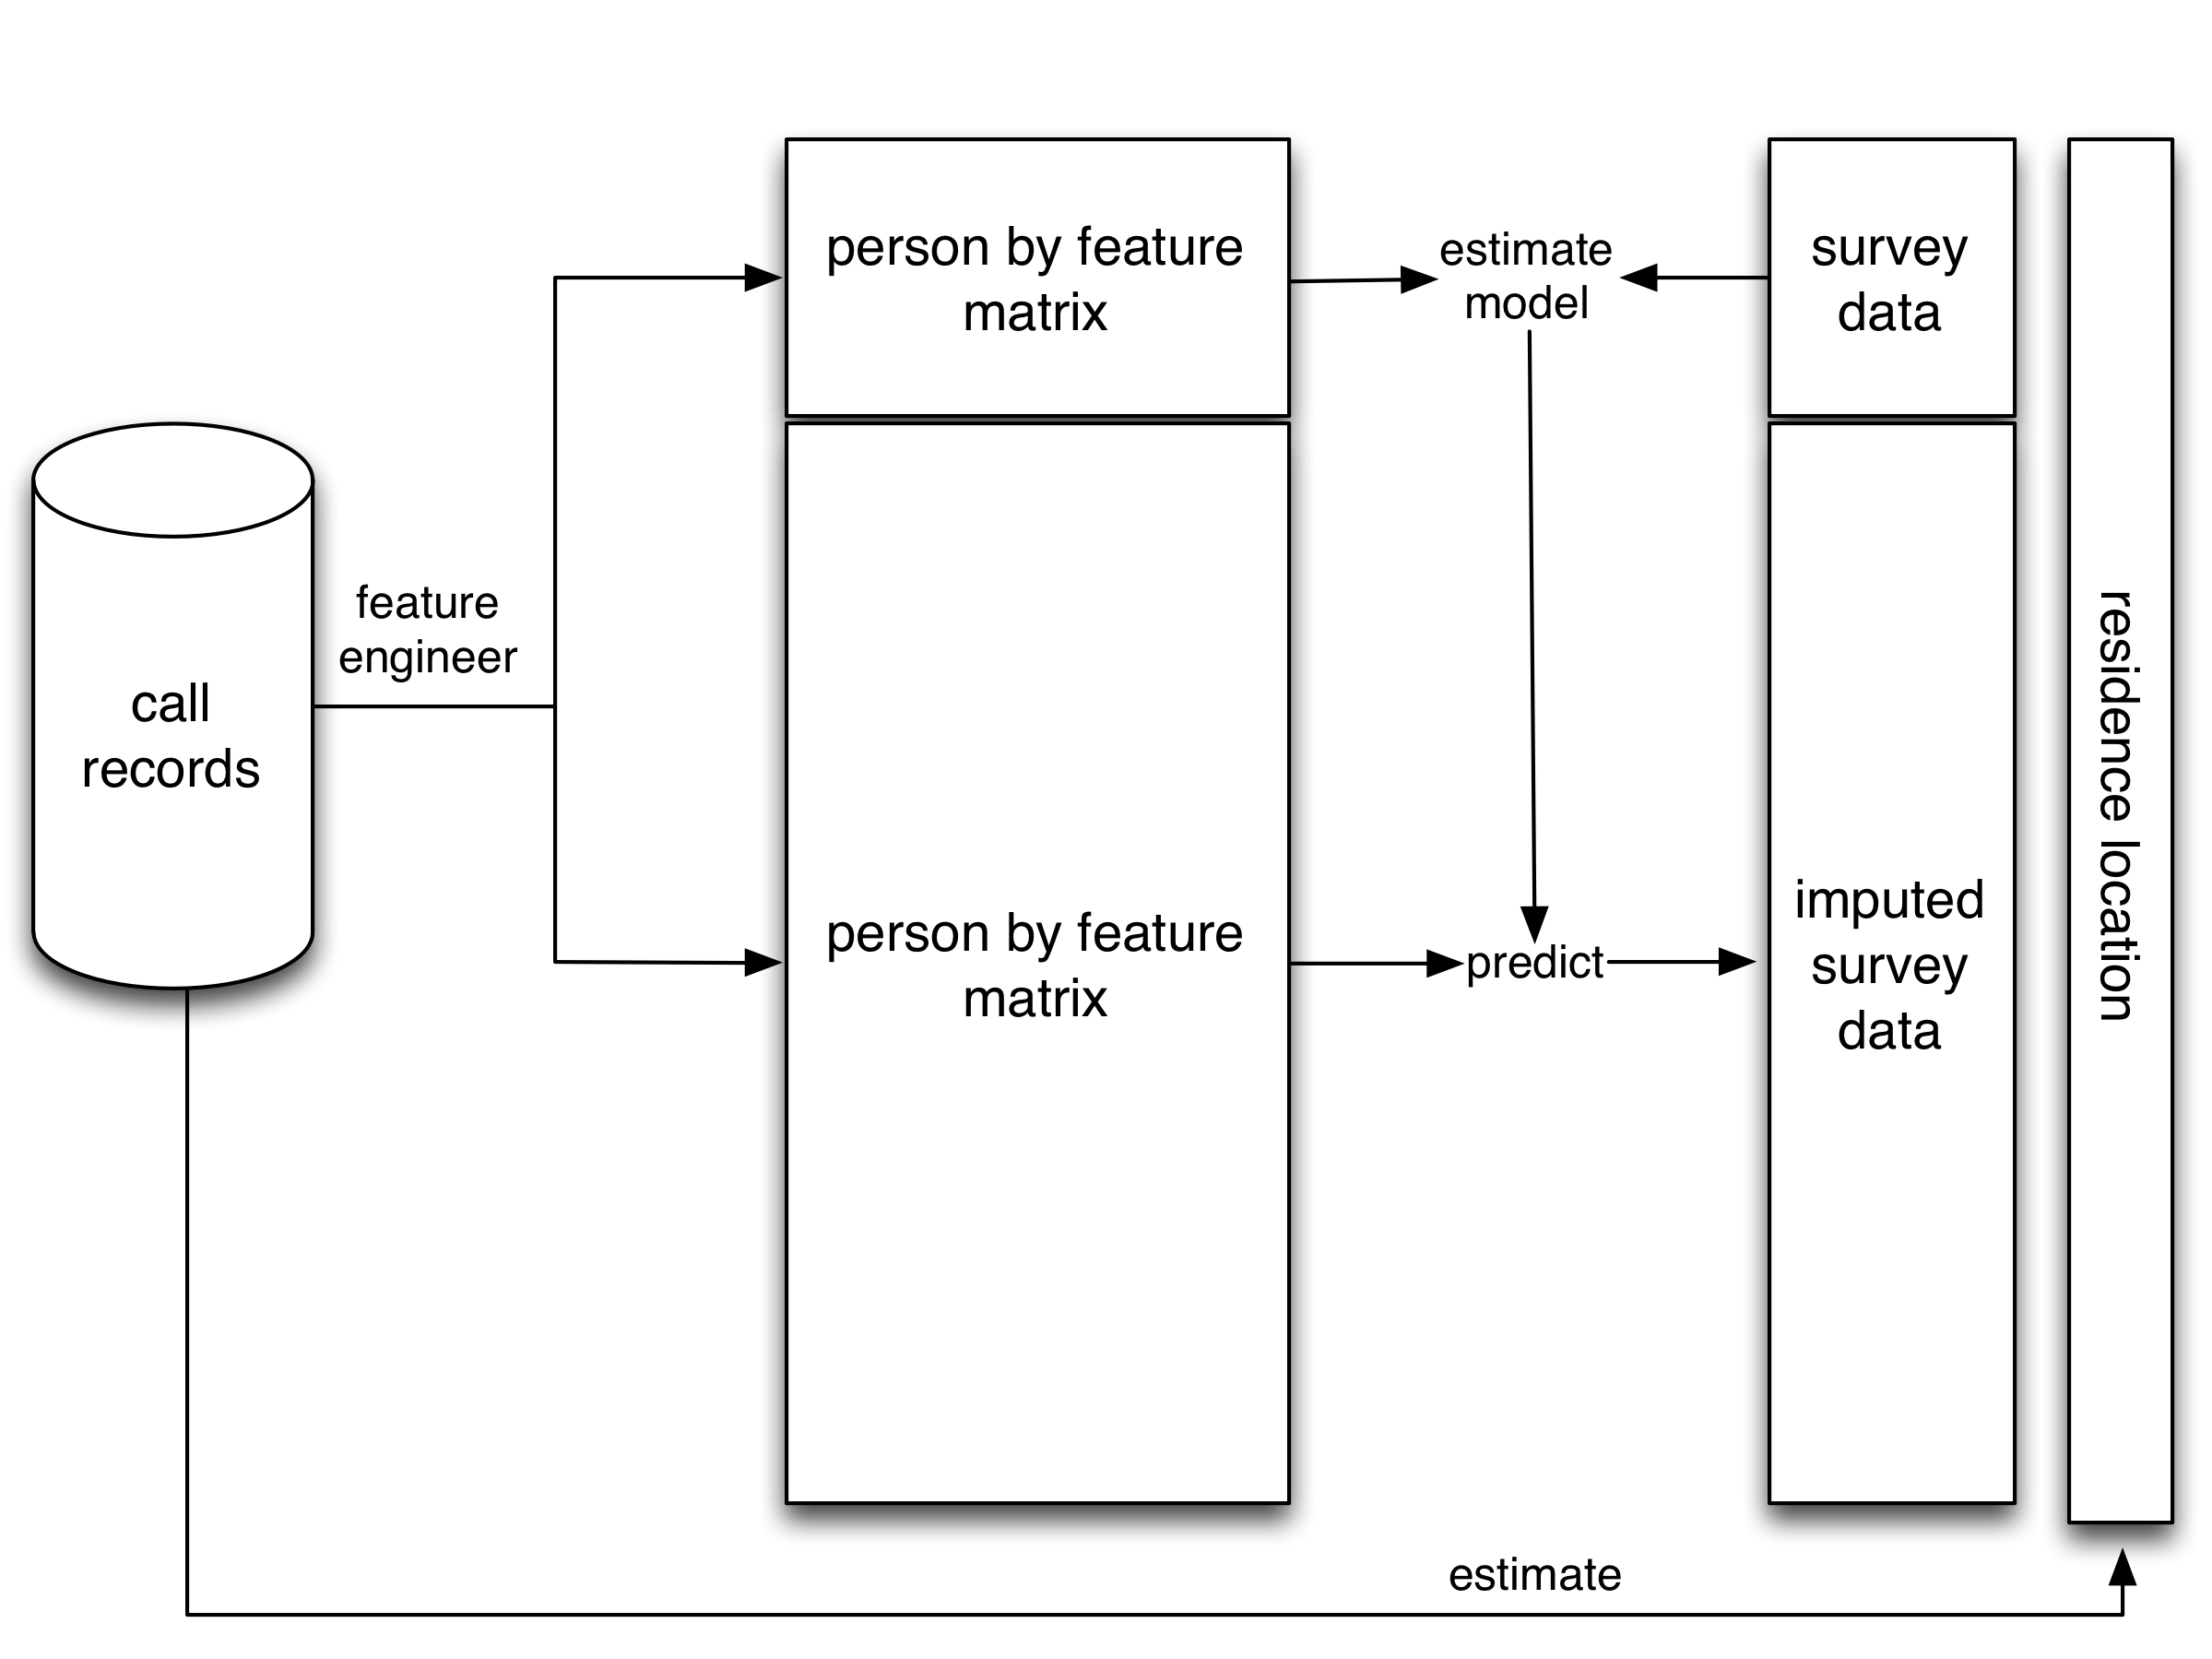
\includegraphics[width=0.7\textwidth]{figures/blumenstock_predicting_2015_schematic_6}}
\end{center}

\end{frame}
%%%%%%%%%%%%%%%%%%%%%%%%%%%
\begin{frame}

\begin{center}
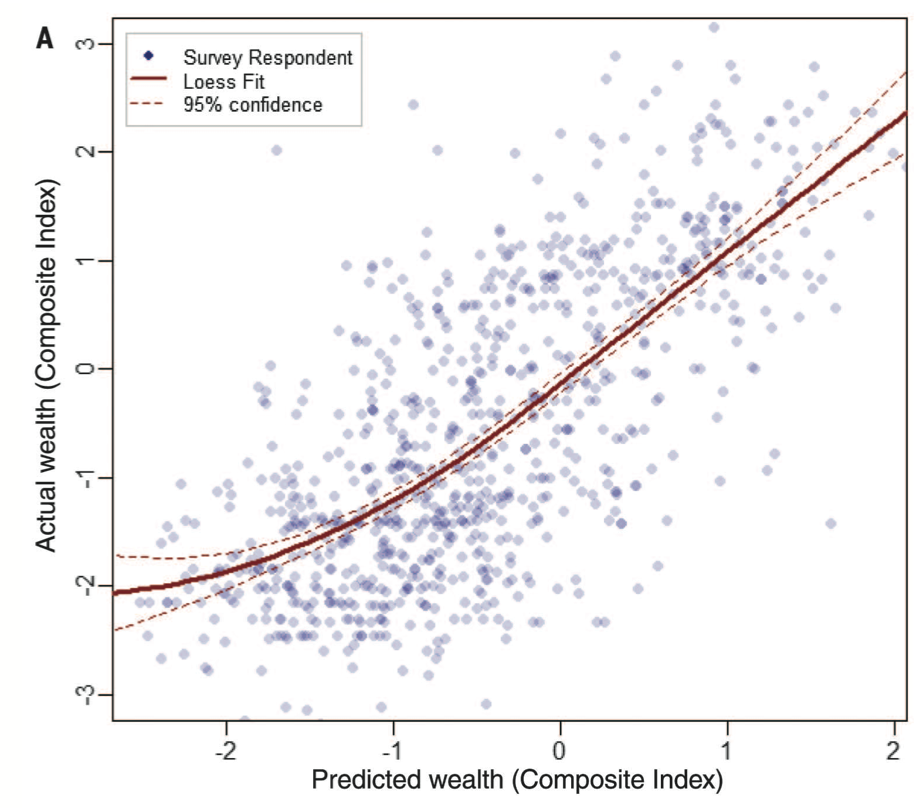
\includegraphics[width=0.7\textwidth]{figures/blumenstock_predicting_2015_fig1a}
\end{center}

\end{frame}
%%%%%%%%%%%%%%%%%%%%%%%%%%
\begin{frame}

\begin{center}
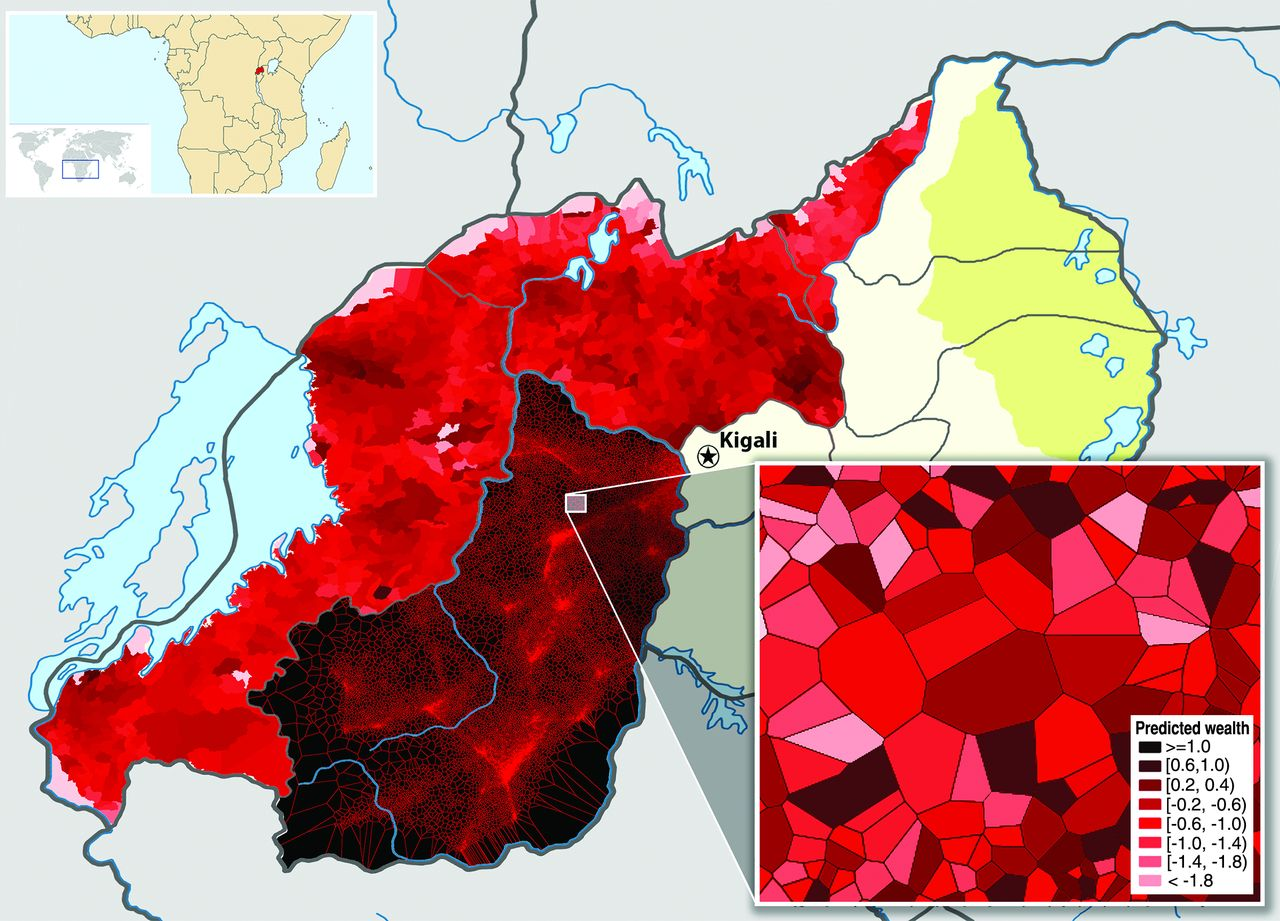
\includegraphics[width=0.7\textwidth]{figures/blumenstock_predicting_2015_fig2}
\end{center}

\end{frame}
%%%%%%%%%%%%%%%%%%%%%%%%%%
\begin{frame}

\begin{center}
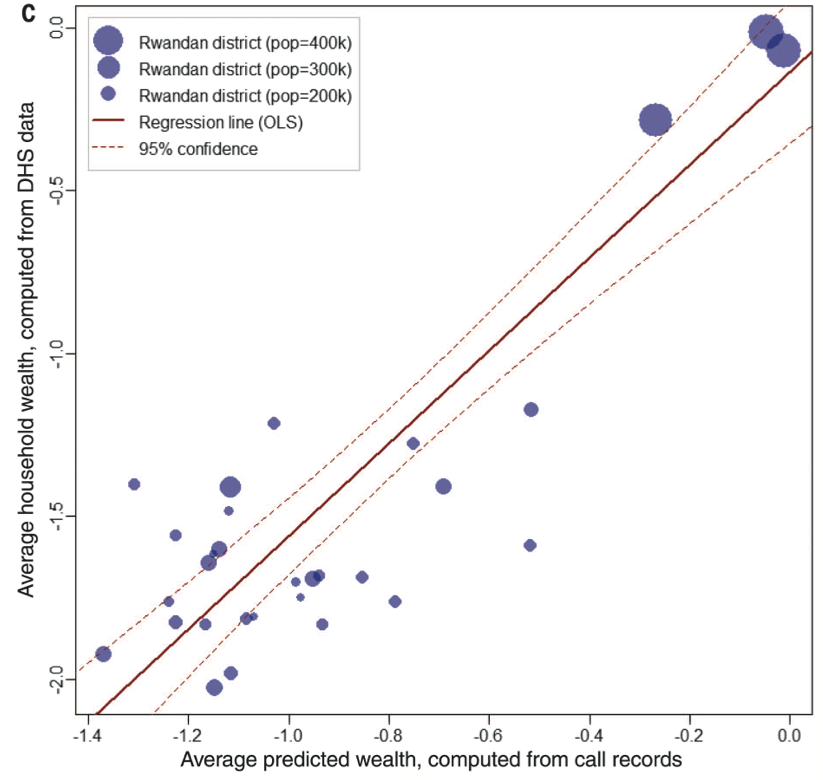
\includegraphics[width=0.45\textwidth]{figures/blumenstock_predicting_2015_fig3c}
\end{center}

\pause

\begin{itemize}
\item 10 times faster
\item 50 times cheaper
\end{itemize}

\end{frame}
%%%%%%%%%%%%%%%%%%%%%%%%%%
\begin{frame}

\begin{center}
\begin{tabular}{ccc}
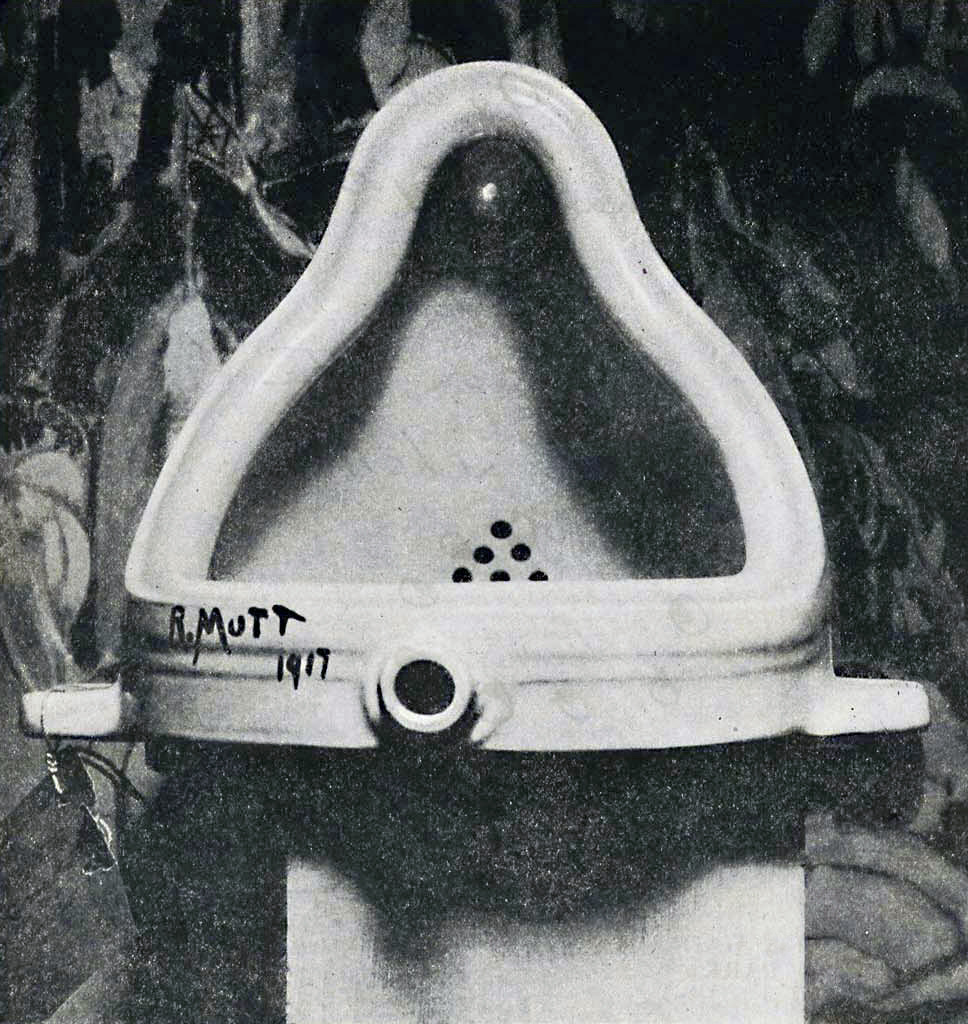
\includegraphics[width=0.30\textwidth]{figures/duchamp_fountain} & \phantom{12} \LARGE{+} \phantom{12} & 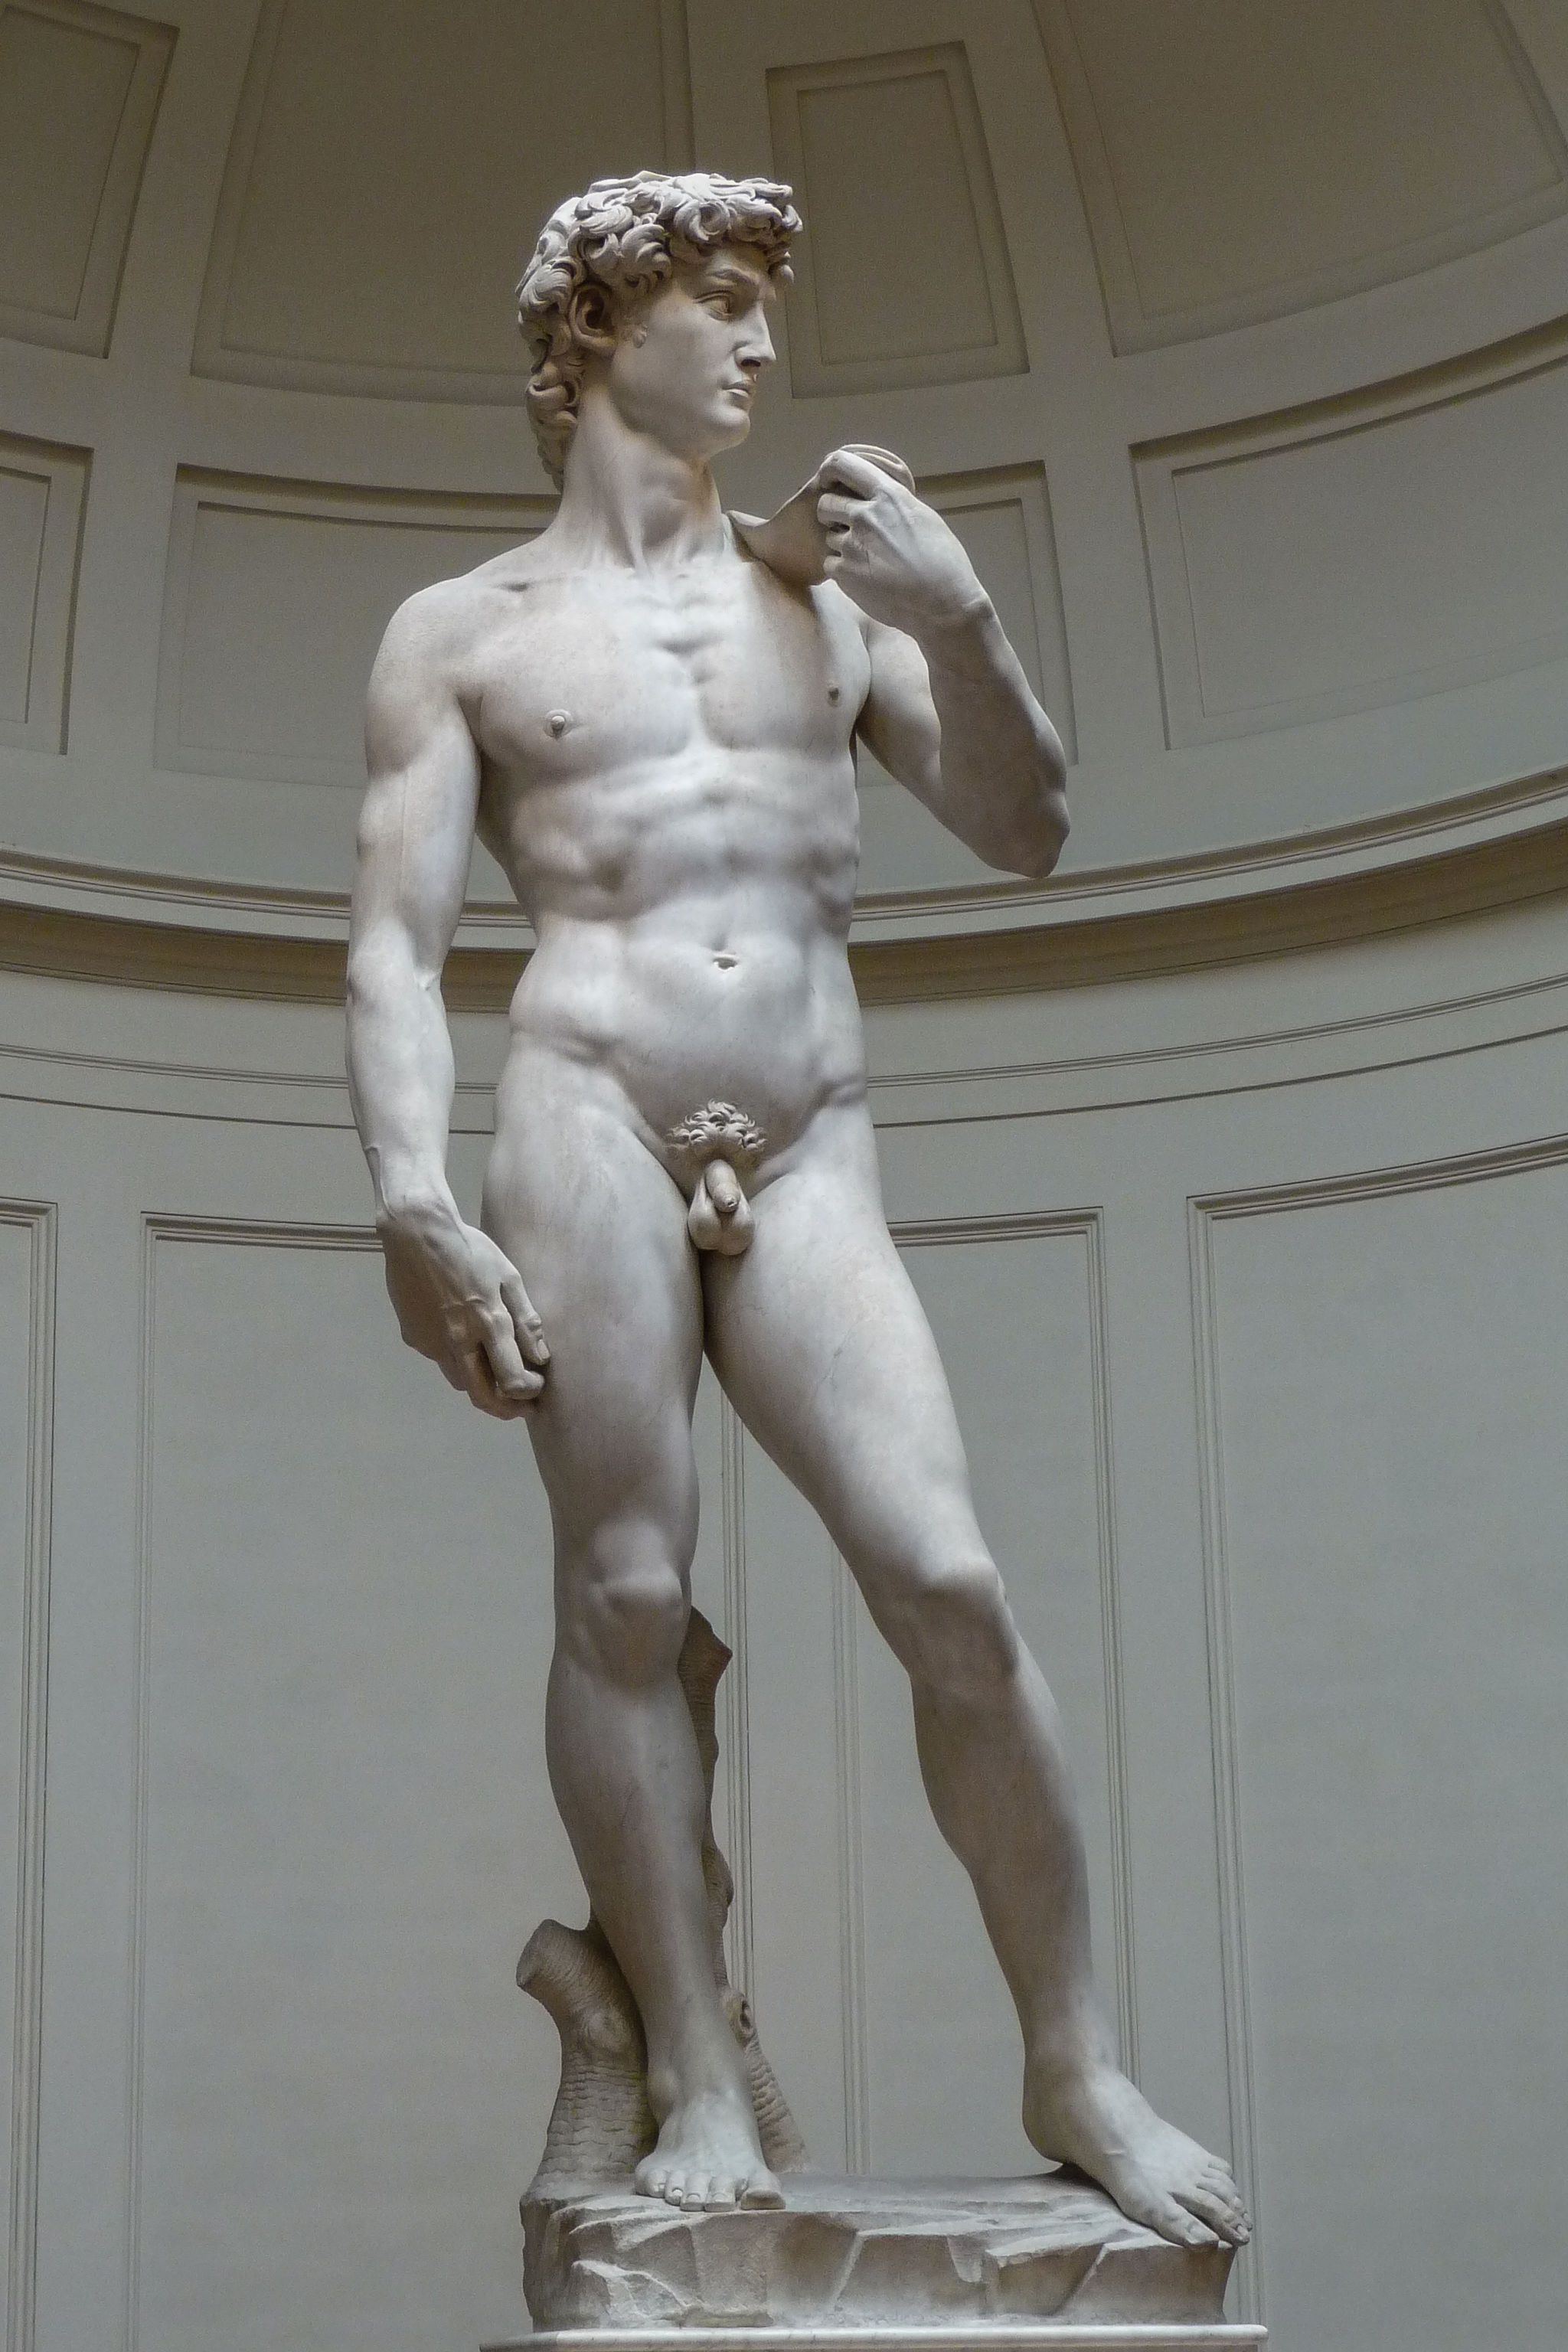
\includegraphics[width=0.30\textwidth]{figures/michelangelo_david} \\
\LARGE{Readymades} &  & \LARGE{Custommades}
\end{tabular}
\end{center}

\vfill
\vspace{0.2in}
\TINY{\url{https://commons.wikimedia.org/wiki/File:Duchamp_Fountaine.jpg}}\\
\TINY{\url{https://commons.wikimedia.org/wiki/File:\%27David\%27_by_Michelangelo_JBU0001.JPG}}

\end{frame}
%%%%%%%%%%%%%%%%%%%%%%%%%%%
{
\usebackgroundtemplate{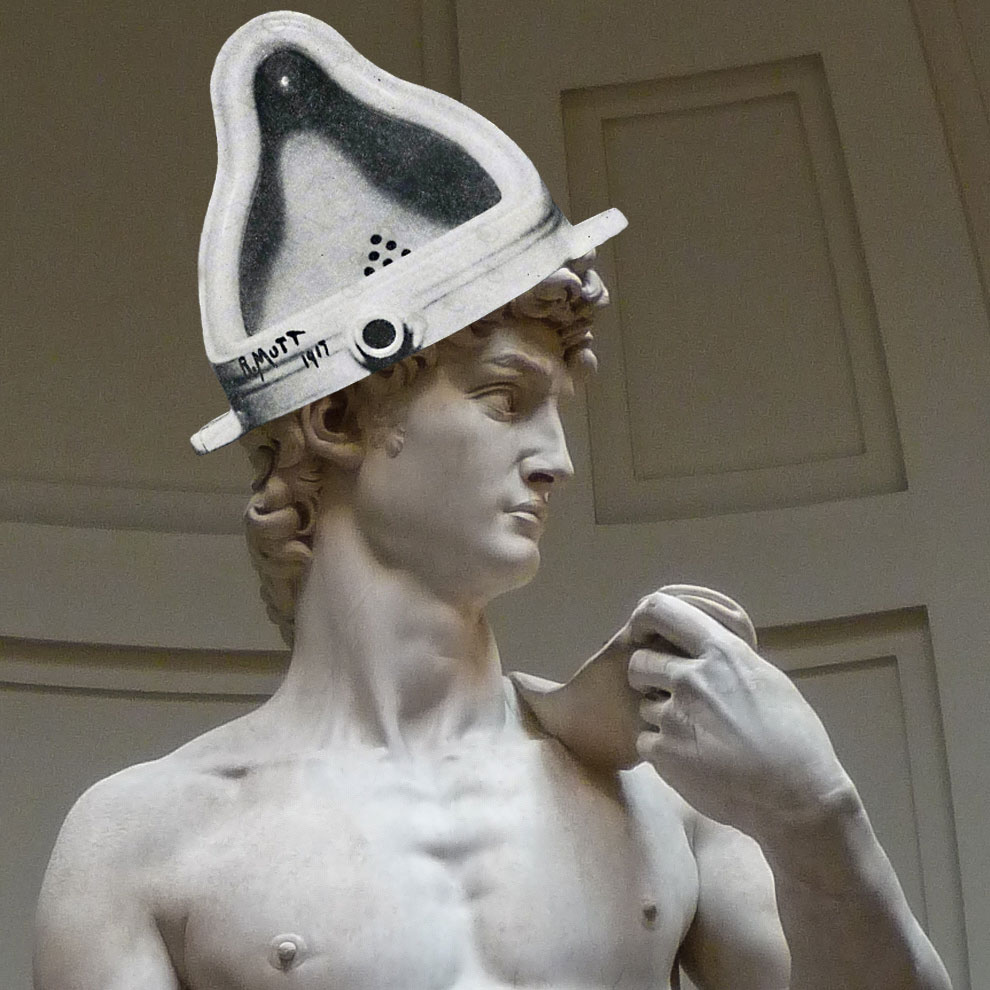
\includegraphics[width=\paperwidth]{figures/custom-david-cropped}}
\begin{frame}[plain]

\vspace{3.58in}
\hspace{-0.32in}
\TINY{Created by Kedron Rhodes}
\end{frame}
}
%%%%%%%%%%%%%%%%%%%%%%%%%%
\begin{frame}

Wrap-up:
\begin{itemize}
\item Surveys and big data are compliments not substitutes
\pause
\item Sometime we do ``enriched asking'' and sometimes ``amplified asking'' (role of big data source is different in both cases)
\pause
\item Learn more: see ``what to read next'' in Ch 3 of \href{https://www.bitbybitbook.com/en/1st-ed/asking-questions/asking-what-to-read-next/}{\textit{Bit by Bit}}.
\end{itemize}

\end{frame}
%%%%%%%%%%%%%%%%%%%%%%%%%%%
\frame{\titlepage}
%%%%%%%%%%%%%%%%%%%%%%%%%%%

\end{document}
